\chapter{Método de trabajo}
\label{chap:metodo}
\drop{T}~ras haber analizado cuales son los objetivos a desarrollar en el TFG, y realizado un análisis de las tecnologías existentes, es necesario asignar una metodología para la gestión del proyecto. 

Para ello, y valorado el número de personas que están involucradas en el proyecto (director del TFG y su autor), se efectúa una investigación sobre cuales son las alternativas de metodologías para llevarlo a cabo, que sea ágil, ligera, y por supuesto, flexible a cambios para adaptar nuevos requisitos que puedan surgir.

Las metodologías Agile, surgen en el año 1990, como herramienta de gestión software que indicase unas correctas directivas para llevar a acabo los proyectos. 

Las metodologías existentes hasta la época, tenían una rigurosa asignación de roles, actividades y artefactos (incluyendo el modelado y una documentación muy detallada), que, no obstante, a día de hoy sigue siendo necesaria para proyectos de gran envergadura, que necesitan una alta gestión de tiempo y recursos. 

Según avanza el desarrollo de aplicaciones software, entran en escena nuevas situaciones en las cuales este tipo de métodos de gestión no encaja totalmente con estas metodologías tradicionales. 

Los métodos Agile promueven una gestión de proyectos, que se basa principalmente en fomentar la constante inspección del trabajo y la adaptación de éste. Se trata de un sistema organizado que facilita el trabajo el equipo, una correcta organización, y favorece el rendimiento del tiempo empleado en el desarrollo.

Scrum fue creado, con las características de estos métodos de gestión, mediante una comunicación directa y haciendo uso de ingeniería concurrente, basándose en las ideas del «Manifiesto por el Desarrollo Ágil de Software» (detalladas en la siguiente sección del documento).

Por lo tanto, basándose en estas ideas, y teniendo en cuenta el número de personas que están involucradas en el proyecto, se ha elegido la metodología de trabajo Scrum.


\section{Metodología Agile}



\section{Scrum como metodología de trabajo}



\subsection{Roles}



\subsection{Artefactos}



\subsection{Motivos de la elección del método Scrum}



\section{Aplicación del método de trabajo}


\subsection{Iteración 1: Inicio del TFG}

Esta iteración tiene como finalidad, conocer el alcance del proyecto y los puntos a tratar en la línea de trabajo, la cual está dedicada al área de electrónica de consumo y lúdico-educativa. 

Establecer una propuesta de Trabajo Fin de Grado, así como los diferentes aspectos relacionados con la organización, planificación y seguimiento del proyecto.

El presente Trabajo Fin de Grado, será dirigido y supervisado como director \textbf{Francisco Moya Fernández}.

\subsubsection{Descripción de la línea de trabajo.}
La propuesta de este TFG consiste en el diseño y prototipado de un sistema electrónico de bajo coste, basado en interfaces tangibles, para aplicaciones lúdico-educativas. Para llevar acabo la plataforma de juego, se hace uso de sistemas empotrados basados en microprocesadores, junto a un conjunto de periféricos, aprovechando la tecnología para facilitar los mecanismos de aprendizaje.
La elección de esta línea de trabajo ofrece la posibilidad de integrar y desarrollar los contenidos, capacidades y habilidades adquiridas durante todo el periodo de docencia en el \textbf{Grado en Ingeniería Electrónica Industrial y Automática}.


\subsubsection{Organización y planificación del proyecto.}
La metodología aplicada a la organización y planificación del proyecto es \emph{Scrum}, la cual divide el proceso del desarrollo del proyecto en varias iteraciones (\emph{Sprints}).
Cada iteración tiene como objetivo realizar una reunión de planificación, donde se definen y analizan las diferentes etapas que componen la evolución del proyecto expuestas como historias de usuario.
Las historias de usuario contienen una descripción corta de las necesidades del proyecto. Cada una de ellas es redactada al final de cada reunión y analizadas al principio de la iteración siguiente.
La duración de tiempo entre iteraciones establecido es de \textbf{dos semanas}. 

\subsubsection{Redacción, seguimiento y desarrollo del trabajo escrito.}
La memoria es redactada mediante el editor de textos \emph{TextMaker} basado en \LaTeX{}, debido a la simplicidad para redactar documentos de forma estructurada.
El trabajo escrito es alojado en un repositorio de la plataforma \emph{github.com} para la supervisión y seguimiento del proyecto. Esto permite visualizar y realizar cambios dinámicos en la memoria por parte del autor y del director del TFG.

\subsubsection{Próximas historias de usuario.}
Al finalizar la primera reunión son establecidas las historias de usuario para la próxima iteración.
\begin{itemize}
\item Estudio y primer análisis del problema.
\item Elaborar una primera propuesta de diseño a partir del análisis previo del problema.
\end{itemize}

\subsection{Iteración 2 : Formación y planificación del TFG. }
Análisis y exposición de las distintas características que definen una plataforma de juego basada en interfaces tangibles. Se seleccionan y destacan aquellos aspectos que serán de utilidad, para ser aplicados a un primer diseño de sistema tangible.\\
Planteamiento y explicación del funcionamiento de la plataforma de juego basada en interacción tangible, tras haber realizado un primer estudio y análisis previo.

\subsubsection{Estudio y primer análisis del problema.}
Localizar y estudiar los principales sistemas basados en interacción tangible, para destacar sus principales características. Para ello, se hace uso de las diferentes bases de datos actualmente disponibles como \emph{Scopus} o \emph{Web Of Science}.

\textbf{Características principales del modelo básico en una interfaz de usuario tangible:}\\
\begin{itemize}
\item Elementos físicos de entrada/salida o control, y representaciones tangibles e intangibles.
\item Información comprensible y literalmente palpable.
\item Acoplamiento de las representaciones tangibles a la información digital latente, mediante la manipulación de objetos que sirven como puente de unión entre el mundo digital y el mundo real. Convertir la información digital en forma física.
\item Equilibrio y fuerte acoplamiento perceptual entre representaciones tangibles e intangibles.
\end{itemize}

\subsubsection{Propuesta de un primer dispositivo de juego a partir de las propiedades en sistemas tangibles.}
La propuesta incorpora las características principales aplicadas a interfaces tangibles, como primera toma de contacto con este tipo de dispositivos.
Estos sistemas, permiten a los niños escribir un programa mediante el uso de objetos físicos, sin hacer uso de un teclado, para posteriormente ver los resultados realizados por ellos mismos.

\textbf{Modelo básico en las interfaces de usuario tangible.}\\
Las propiedades más importantes en la interfaz entre personas e información digital son:
\begin{itemize}	
\item Elementos de entrada/salida o control
\item Representación tangible de la información digital como mecanismo de control físico interactivo directo. 
\item Representación intangible como herramienta de acoplamiento entre la realización física y la información digital.
\end{itemize}

\textbf{Descripción.}\\
El objetivo del juego es realizar una secuencia (propuesta por la propia aplicación o creada por el niño), a partir de elementos tangibles, que corresponden a unas instrucciones específicas, como pueden ser movimientos, representaciones gráficas, salidas acústicas, etc. El resultado de la secuencia es mostrado de manera gráfica en otro dispositivo.\\
Existen dos modos de funcionamiento dentro de la aplicación. El niño puede crear una secuencia aleatoria con los elementos tangibles para obtener una salida gráfica, o de manera inversa, proponer gráficamente al niño que realice una secuencia con los elementos tangibles.
 
El modelo propuesto incorpora las características básicas de las interfaces de usuario tangible, y presenta
dos tipos de componentes principales:
\begin{itemize}
\item \textbf{Placa principal:} procesa y muestra gráficamente, las instrucciones recibidas del resto de componentes (elementos tangibles de entrada/salida). La comunicación con el resto de los elementos es ejecutada por una red inalámbrica de comunicaciones \emph{WiFi}.
\item \textbf{Elementos de entrada/salida:} corresponden a la representación intangible de la información digital. 
Está formado por una serie de bloques de pequeñas dimensiones y estructura cúbica. Estos cubos son conectados
entre sí, para formar una secuencia. Cada elemento se comunica con el anterior, con un conector magnético \emph{micro USB}.
Cada cubo esta diferenciado por código de colores, para una interacción más intuitiva, e incluyen un indicador visual (\emph{led RGB}), para indicar en que momento de la secuencia se encuentra.
Las instrucciones son enviadas a la placa principal vía inalámbrica para ser procesadas.
Cada elemento lleva a cabo únicamente una función. Existen tres funciones principales:
\begin{itemize}
\item \textbf{Elemento de inicio.} Elemento principal de control imprescindible para poder crear una secuencia (ver Figura ~\ref{fig:Elementoinicio}).
Incorpora un microcontrolador el cual maneja un módulo de comunicaciones inalámbricas Wifi, para el intercambio de información con la placa principal.
Dispone de un pulsador para iniciar la secuencia.
El resto de los elementos tangibles deben ser conectados en \emph{serie} a este módulo para establecer comunicación.

\item \textbf{Elemento de eventos.} Genera un evento dentro de la secuencia (desplazamientos, temporizador, indicador luminoso, acústico, ...).
\item \textbf{Elemento repetición.} Al situarse al final de una secuencia, retoma el inicio de esta (vuelve al elemento de inicio).
\end{itemize}
\end{itemize}

\begin{figure}[!h]
\begin{center}
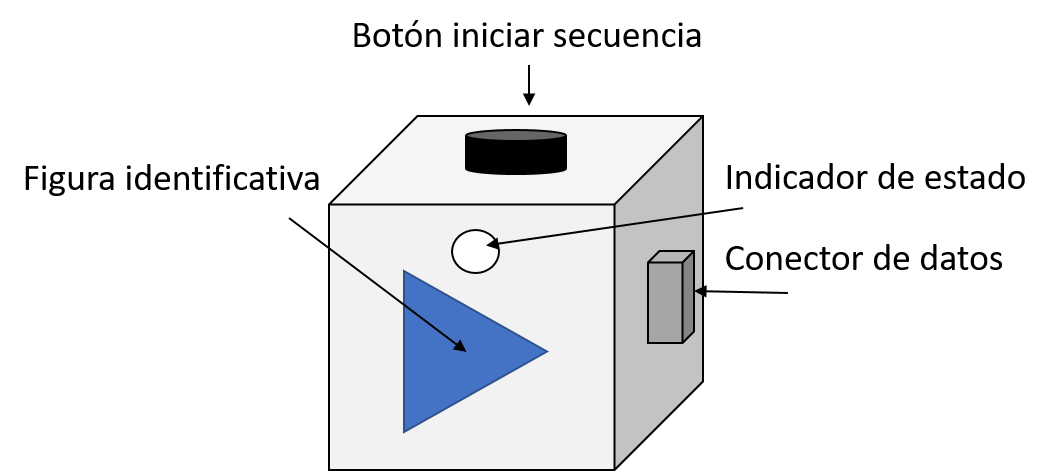
\includegraphics[width=0.7\textwidth]{Propuesta1Inicio.png}
\caption{Diseño del elemento tangible \emph{inicio}.}
\label{fig:Elementoinicio}
\end{center}
\end{figure}

\begin{figure}[!h]
\begin{center}
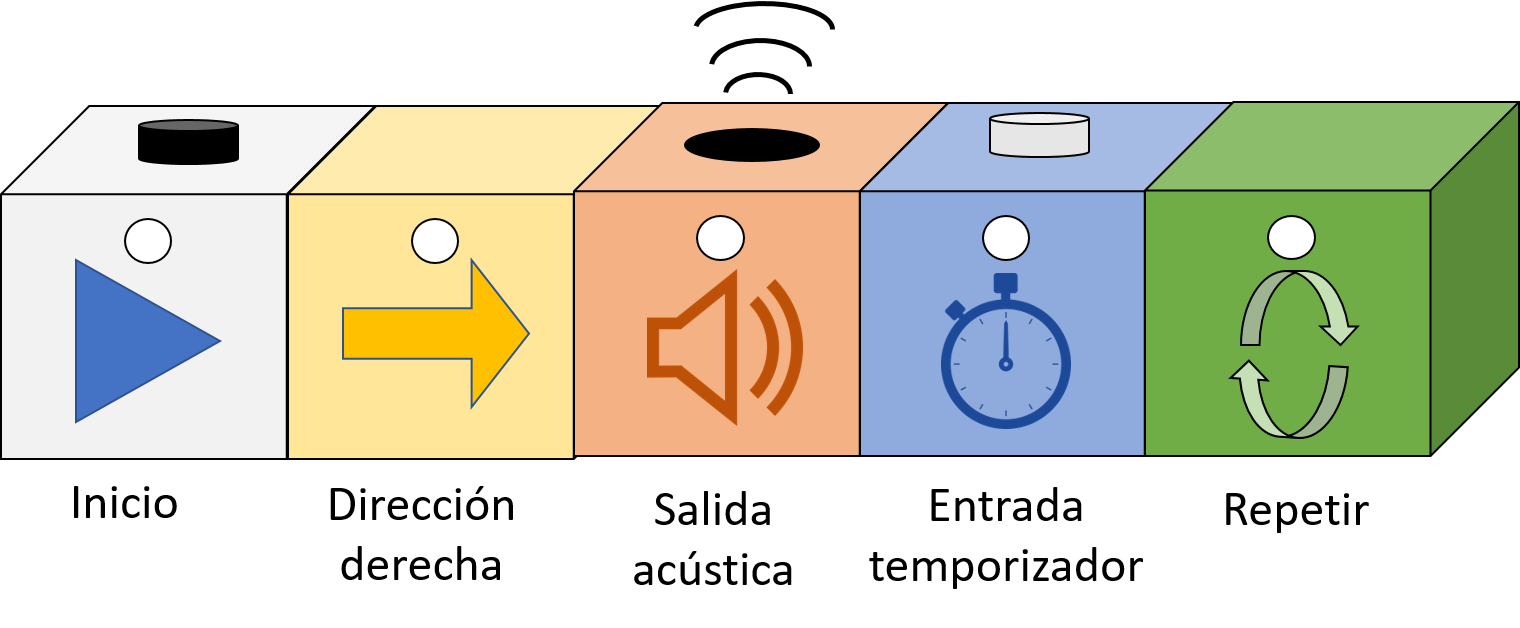
\includegraphics[width=0.7\textwidth]{Propuesta1Secuencia.png}
\caption{Ejemplo de secuencia. Al pulsar el botón \emph{iniciar secuencia}, se produce un desplazamiento hacia la derecha. A continuación, se genera una señal acústica. La secuencia se mantiene durante un tiempo en pausa (según el tiempo ajustado en el temporizador). Finalmente se repite la secuencia.}
\label{fig:Secuencia}
\end{center}
\end{figure}

Las comunicaciones entre módulos son realizadas por medio de un conector magnético \emph{micro USB} que facilita la conexión entre los mismos. Existen 4 líneas de comunicación serie (entrada de datos, salida de datos, habilitación y señal de reloj). Incorpora un \emph{registro de desplazamiento} y un \emph{multiplexor} para el manejo de datos (Figura ~\ref{fig:Registros}).
La trama de datos consta de 8 bits. Los 3 bits más significativos, identifican el tipo de instrucción asignada al cubo. El resto de los bits son utilizados para la iluminación de un \emph{led RGB}, que indica el estado de la secuencia.

La Figura ~\ref{fig:Secuencia} muestra un ejemplo de una posible secuencia.

\begin{figure}[!h]
\begin{center}
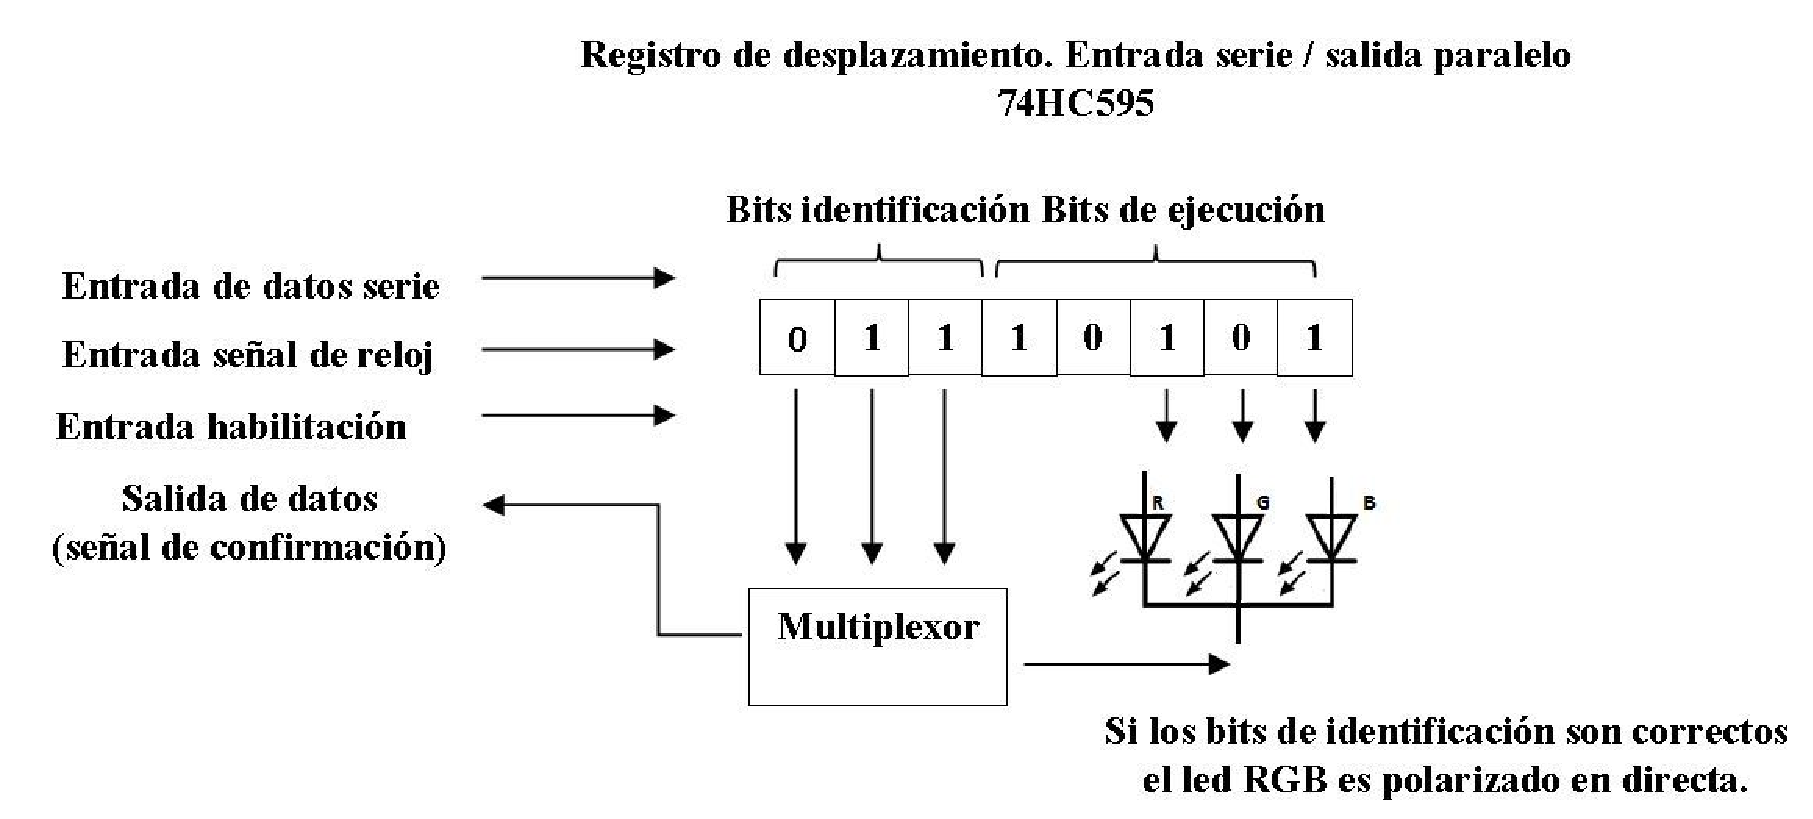
\includegraphics[width=0.7\textwidth]{Propuesta1registros.pdf}
\caption{Diseño del manejo de datos en los elementos tangibles mediante registro de desplazamiento y multiplexor.}
\label{fig:Registros}
\end{center}
\end{figure}


\textbf{Análisis de la primera propuesta de diseño}\\
La primera propuesta de diseño es analizada junto con el director del proyecto, quedando descartada. 
En el mercado existen dispositivos de características muy similares, no aportando nada destacable. Los conectores magnéticos no cumplen la normativa vigente para dispositivos en este tipo de aplicaciones, siendo peligroso para los niños.
Se concreta conocer en profundidad el alcance del proyecto, entendiendo que hay que construir, realizando un estudio más amplio sobre los actuales sistemas enfocados a la programación tangible, tecnología y características. Identificar los puntos a mejorar en los actuales sistemas y contribuir a mejorarlos, diseñando una plataforma de juego que resuelva esos puntos. El análisis permite establecer unos requisitos de diseño.




\subsubsection{Próximas historias de usuario.}

\begin{itemize}
\item Estudio avanzado del problema. Revisión sistemática (recopilación de información).
\item Identificar áreas de mejora en los actuales sistemas tangibles.
\item Selección de las áreas de mejora para la redacción de los objetivos.
\item Elaborar una segunda propuesta de diseño a partir del estudio avanzado del problema y de las áreas de mejora.

\end{itemize}


\subsection{Iteración 3: Estudio avanzado del problema. Identificación y selección de las áreas de mejora en sistemas tangibles.}

Determinar cuáles son los principales sistemas con interfaz tangible aplicados a la programación para niños, obteniendo las ventajas y desventajas, así como las principales características y tecnología utilizada en cada uno de ellos.
Segunda propuesta de diseño de plataforma de juego haciendo uso del análisis desarrollado en esta iteración.



\subsubsection{Estudio avanzado del problema.}


Estudiar los diferentes enfoques que aportan los dispositivos actuales basados en interfaces tangibles. Destacar los sistemas aplicados al aprendizaje de la programación para niños. Análisis de las distintas tecnologías que utilizan.
Recopilar información relevante referida al tema tratado. Posteriormente, elaborar un capítulo dedicado a las distintas plataformas y dispositivos que emplean este tipo de interfaces, referenciando las fuentes consultadas en cada caso.

En el \textbf{Capítulo Antecedentes \ref{chap:antecedentes}} de este documento, se muestran los resultados sobre los principales estudios experimentales aplicados a la interacción tangible, y como motiva a niños de tempranas edades en sus habilidades computacionales.\\

En ese capítulo, se indican los dispositivos que han sido utilizados para el aprendizaje computacional más importantes, destacando los diferentes enfoques que aportan cada uno de ellos en la interacción tangible.

\textbf{Estudios experimentales sobre Interacción tangible.}

A continuación, se exponen a modo de resumen, las citas más importantes destacadas por los distintos autores, en los artículos analizados:
\begin{itemize}
\item Exponer a los niños en edades tempranas a un pensamiento computacional, ayuda a construir una base sólida en la mecánica de programación de computadoras \cite{Grover}.

\item El entorno de programación debe motivar fuertemente al usuario, colocándolo en un contexto que sea convincente y significativo, para que no se dé por vencido \cite{Ishii}.

\item Manipular objetos con las manos en lugar de modelos mentales, puede cambiar la forma en la que un niño recuerda y recupera la información enseñada \cite{Piaget}.

\item Las interfaces digitales se convierten en poderosas herramientas de aprendizaje cuando los niños se convierten en creadores en lugar de sólo consumidores de contenido digital \cite{Resnick}. 

\item Al programar, los niños exploran los conceptos fundamentales de secuenciación, reconocimiento de patrones y relaciones de causa y efecto. Los niños aprenden a contar una historia de principio a fin, realizar secuencias de números y letras, formas o colores \cite{Kazakoff}.

\item Aprovechan las estrategias de aprendizaje kinestésico natural de los niños para hacer que los conceptos abstractos sean accesibles e intuitivos \cite{Xu}. 

\item Los sistemas tangibles tienen el prometedor potencial de ayudar a los niños a cultivar un cierto conocimiento del pensamiento computacional como abstracción, automatización, descomposición de problemas y análisis \cite{Wang_2015}.

\item Mientras los niños juegan, se involucran con el mundo físico haciendo uso de sus cinco sentidos \cite{Vygotsky}.

\item La interfaz tangible y la interfaz gráfica proporcionan un andamio estratificado a los niños mientras avanzan hacia un entorno de programación cada vez más auténtico \cite{Horn}. 

\item Los sistemas tangibles aplicados en la programación, fomentan el aprendizaje y el rendimiento en tareas computacionales \cite{Sapounidis}.

\item Los niños pequeños aprenden mejor mientras manipulan y transforman activamente materiales reales \cite{Beaty}.

\item La programación, depuración, el acto de construir un sistema, encontrar problemas y resolverlos, es la manera más eficaz de que un niño aprenda \cite{Papert}.

\item Las experiencias motrices, sirven de base para la posible creación de un instrumento cognitivo \cite{Zimmer}.  

\item Existe una interrelación entre la actividad motora y un mayor desarrollo intelectual \cite{Zahner}.

\end{itemize}

\textbf{Conceptos clave aplicados a la programación tangible para niños, extraídos de los diferentes estudios}:
\begin{itemize}
\item \textbf{Abstracción:} La capacidad de abstracción consiste en encontrar el nivel adecuado de detalle para definir y resolver un problema. \cite{Heureux}.
\item \textbf{Automatización:} Proceso por el cual se produce un ahorro de trabajo que se instruye para efectuar un conjunto de tareas repetitivas mediante una computadora. Es mucho más eficiente en comparación con el poder de procesamiento de un ser humano, por lo que las ejecuciones automatizadas de procesos realizados por máquinas simplifican el trabajo \cite{Guzdial}.
\item \textbf{Descomposición y análisis de problemas:} La descomposición puede tomar la forma de desmontar un problema a lo que se cree que es su esencia fundamental \cite{Lee}. Romper los problemas en partes más pequeñas para poder resolverlos y analizarlos de una manera más fácil, ayuda a la simplificación y resolución de problemas más complejos y de mayor escala.
\item \textbf{Creatividad:} La creatividad es a la vez una capacidad integral de los seres humanos y una parte importante del conjunto de actividades del pensamiento computacional \cite{Curzon}. Se intenta desarrollar la habilidad creativa de los niños estimulando su curiosidad, especialmente la imaginación.
\end{itemize}



\subsubsection{Identificar áreas de mejora en sistemas tangibles.}

Identificar y seleccionar las áreas de mejora en dispositivos tangibles, a partir de la información recopilada. Esta información es de gran importancia para poder elaborar una lista de requisitos iniciales para la plataforma de juego.
Las áreas de mejora localizadas son aplicadas en el diseño de una segunda propuesta de interfaz tangible.

Los diferentes sistemas de interacción tangible tienen como propósito general, que la información
sea comprensible y literalmente captable, haciendo uso de objetos físicos que sean
manipulables de una forma natural.

La evolución de la tecnología aplicada a los modelos actuales de sistemas tangibles, van
adaptándose para mejorar los diseños y conseguir de esta forma sistemas más fiables. No
obstante, existen diferentes áreas de mejora localizadas sobre los diferentes sistemas de interacción
tangible:

\begin{itemize}

\item \textbf{Uso de elementos externos para su funcionamiento.} En determinados juegos, es imprescindible
el uso de un ordenador para su normal funcionamiento (como es el caso de \emph{Scratch
\& WeDo}). El uso de periféricos o el uso de una cámara para el reconocimiento de imágenes.

\item \textbf{Elevado número de elementos tangibles para el desarrollo del juego.} Si bien es cierto
que uno de los puntos más importantes a la hora de la programación tangible para niños, es
poder representar partes de código de diferentes elementos tangibles, un gran número
de elementos puede suponer un problema para el niño a la hora del desarrollo del
juego, pudiendo en algunos casos, confundirlo.

\item \textbf{Enfoque exclusivo de un rango de edades para el juego.} En la mayoría de los casos, los
juegos están enfocados a niños de un determinado rango de edades, limitando de esta
manera el juego, al resultar de una dificultad elevada para niños de corta edad, o demasiado fáciles para el resto de las edades.

\item \textbf{Diseño estático del juego.} Una de las limitaciones de todos los juegos que hacen uso
de interfaces tangibles, es que no pueden ser actualizados, o no disponen de actualizaciones
de software, por tanto, el juego no evoluciona, e imposibilita posibles futuras mejoras en los juegos.

\item \textbf{Alto coste de los bloques o dispositivos de realimentación.} El uso de un gran número
de elementos para la interacción tangible eleva el precio del diseño.

\end{itemize}

\subsubsection{Segunda propuesta de plataforma de juego.}

Propuesta de diseño, de un dispositivo o plataforma de juego, en base al modelo básico de interfaces tangibles, que cumpla los requisitos identificados en las distintas áreas de mejora localizadas en esta iteración.\\
Identificar cual es la tecnología más adecuada a utilizar en el dispositivo una vez analizada la evolución tecnológica aplicada a los modelos actuales.\\

Este sistema de programación tangible consta de dos dispositivos. Uno principal y otro de control. El objetivo del juego es realizar programas secuenciales, los cuales son representados en la pantalla del dispositivo principal. Estos programas pueden ser creados o modificados, usando el dispositivo de control, que actúa como elemento tangible.\\

La plataforma de juego se basa en los conceptos de secuenciación, repetición de bucles, y programación creativa.

\begin{itemize}
\item \textbf{Dispositivo principal}: indica todas las operaciones a realizar, ya sea movimientos, secuencias, eventos acústicos, etc. Dispone de una pantalla táctil donde se visualiza y establece el desarrollo del juego. La estructura alberga el sistema de control, comunicación y procesamiento de datos (\emph{Raspberry Pi}). Incorpora sensores de proximidad situados en las cuatro caras que rodean el dispositivo. Dispone de un magnetómetro, cuya finalidad es detectar el dispositivo auxiliar en una posición concreta (encima de la pantalla o en las proximidades del dispositivo principal). La Figura ~\ref{fig:Cuboprincipal} muestra el diseño del dispositivo principal.

\begin{figure}[!h]
\begin{center}
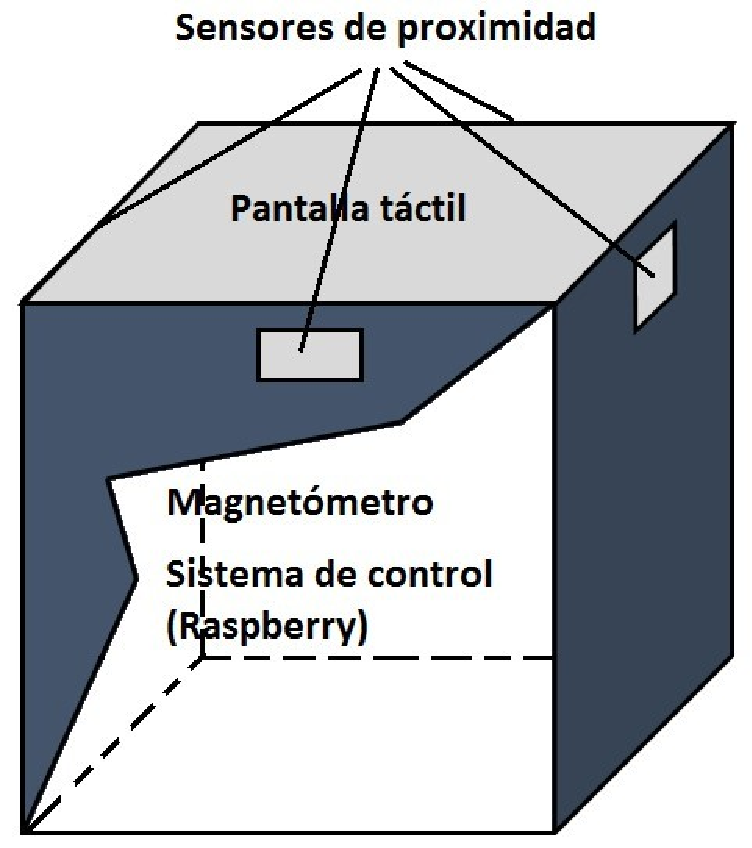
\includegraphics[width=0.5\textwidth]{Propuesta2cuboprincipal.pdf}
\caption{Diseño del dispositivo principal en la segunda propuesta de plataforma de juego.}
\label{fig:Cuboprincipal}
\end{center}
\end{figure}

\item \emph{Dispositivo auxiliar}: es diseñado con el propósito de manipular el programa, para la adicción, reorganización, y eliminación de partes de la secuencia (estructuras de control de flujo, acciones y parámetros). Estas órdenes son representadas en la pantalla táctil del propio dispositivo. La interacción ocurre cuando se sitúa el elemento de control sobre la pantalla del dispositivo principal. Incorpora un giroscopio que posibilita el control de movimiento de la secuencia en determinadas etapas del juego. La Figura ~\ref{fig:Cuboaux} muestra el diseño del dispositivo de control.

\begin{figure}[!h]
\begin{center}
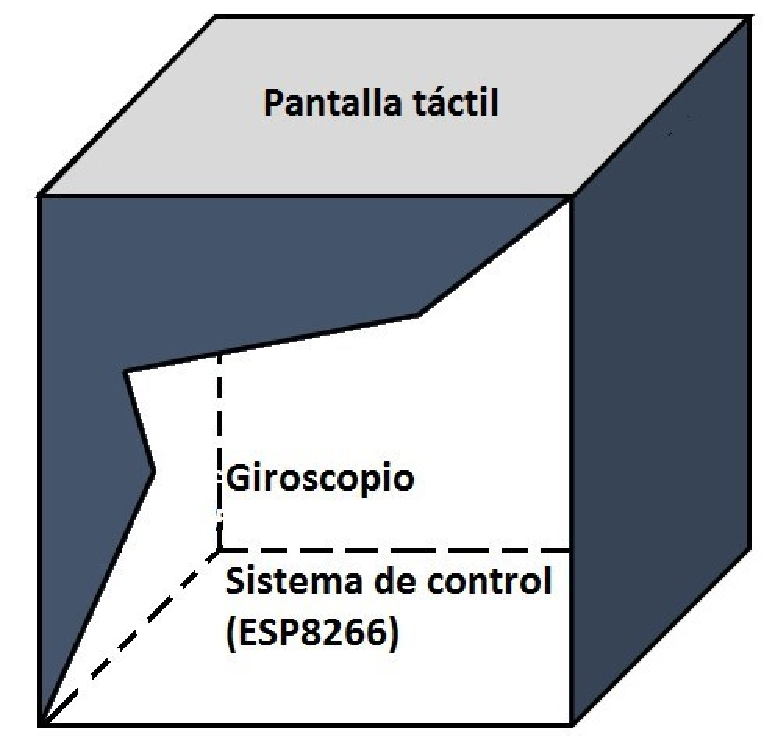
\includegraphics[width=0.5\textwidth]{Propuesta2cuboaux.pdf}
\caption{Diseño del dispositivo de control en la segunda propuesta de plataforma de juego.}
\label{fig:Cuboaux}
\end{center}
\end{figure}
 
\end{itemize}

\textbf{Ejemplos de aplicaciones dentro de la plataforma de juego.}\\
Son implementados los diferentes sensores en la plataforma de juego. Se emplean colores para simplificar la explicación.\\

\textbf{Definir una secuencia.} La pantalla del cubo principal se divide en nueve secciones para que la interacción sea más intuitiva. Se define el recorrido que tendrá la secuencia del juego, deslizando el dedo sobre la superficie de la pantalla (Figura ~\ref{fig:Secuencia1}).

\begin{figure}[!h]
\begin{center}
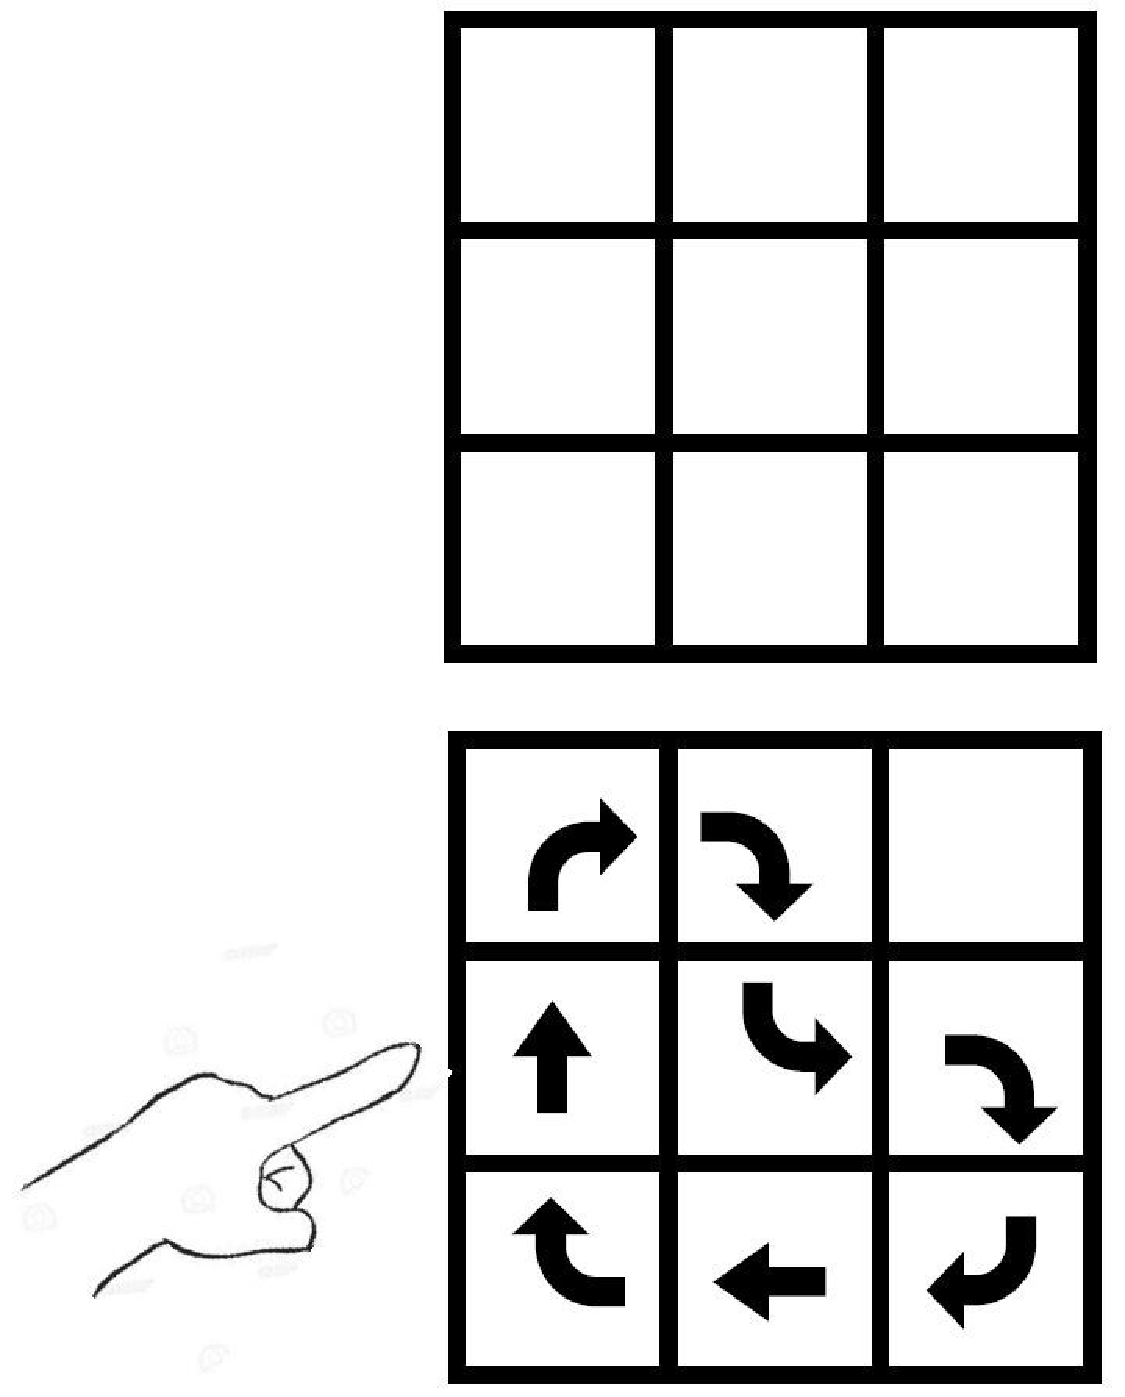
\includegraphics[width=0.5\textwidth]{Propuesta2secuencia1.pdf}
\caption{Definir una secuencia en el dispositivo principal.}
\label{fig:Secuencia1}
\end{center}
\end{figure}


El programa comienza a ejecutarse en función del recorrido marcado, desplazándose de un cuadro a otro (Figura ~\ref{fig:Secuencia2}). 
\begin{figure}[!h]
\begin{center}
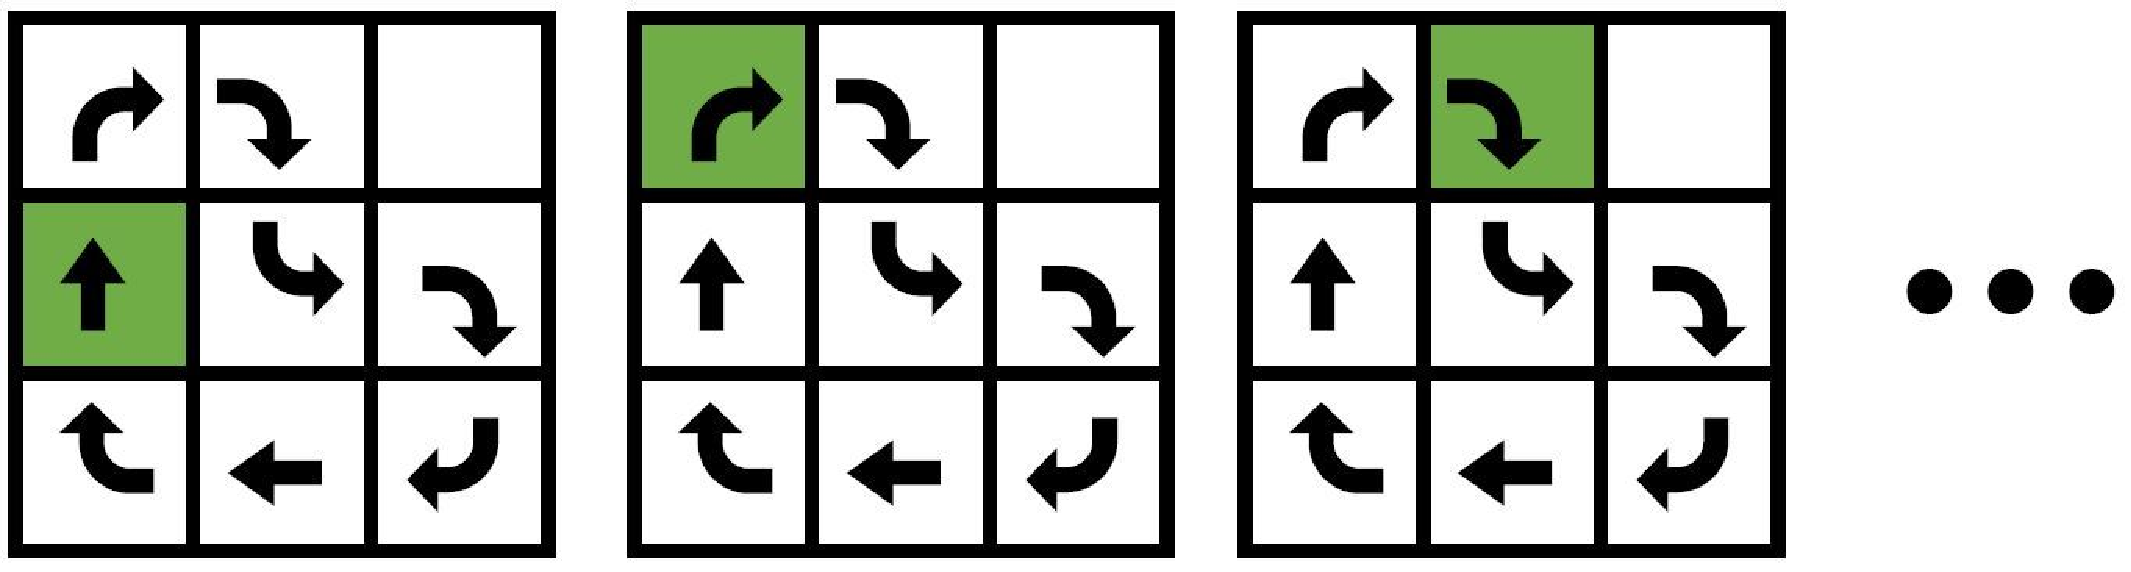
\includegraphics[width=0.5\textwidth]{Propuesta2secuencia2.pdf}
\caption{Desarrollo de una secuencia en el dispositivo principal.}
\label{fig:Secuencia2}
\end{center}
\end{figure}

\textbf{Uso de sensores de proximidad.} Aproximando la mano en los laterales del dispositivo principal, el cuadro es desplazado, siendo la secuencia alterada (Figura ~\ref{fig:Secuencia3}).

\begin{figure}[!h]
\begin{center}
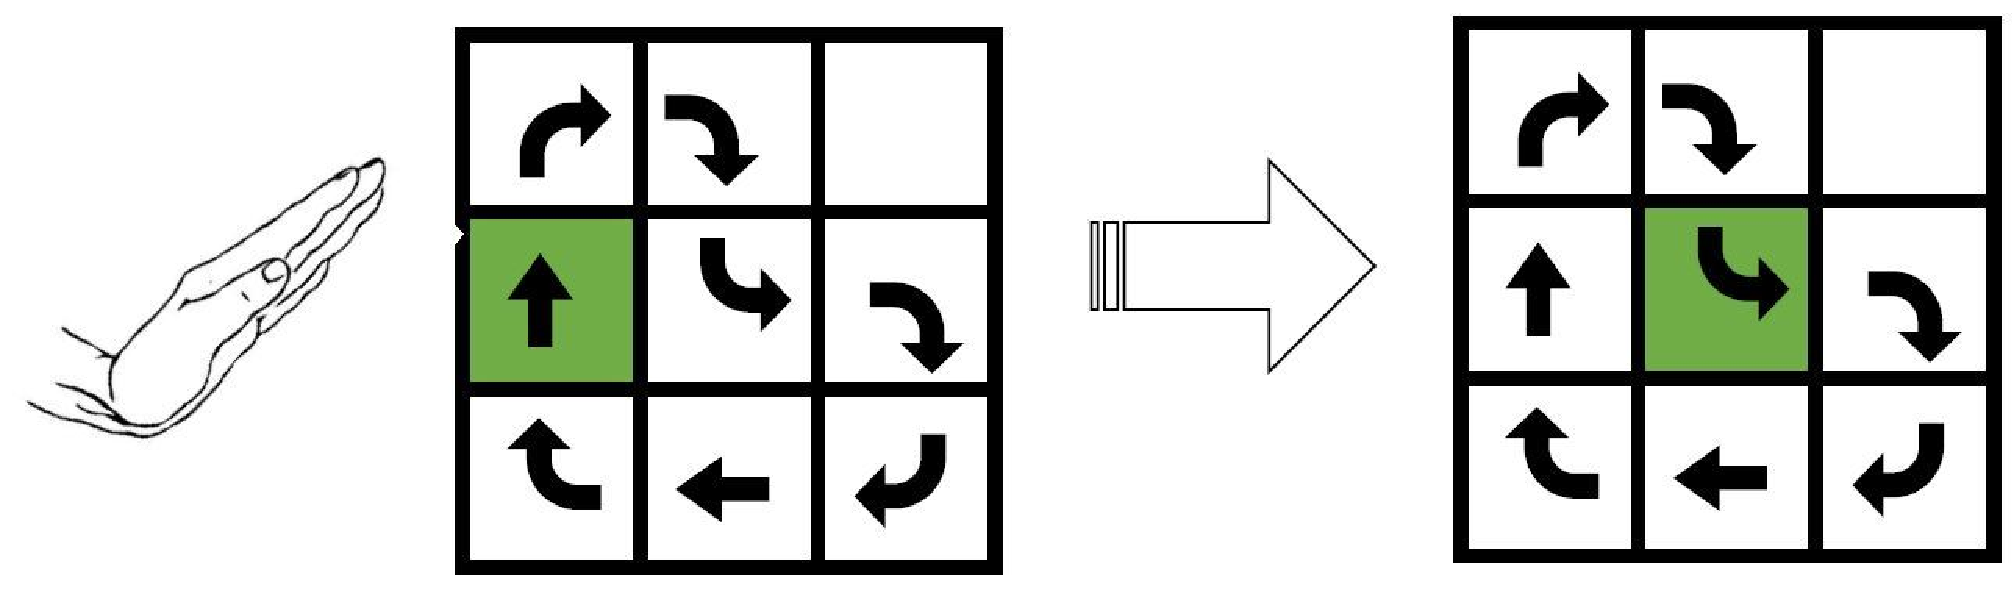
\includegraphics[width=0.5\textwidth]{Propuesta2secuencia3.pdf}
\caption{Modificación de la secuencia usando sensores de proximidad.}
\label{fig:Secuencia3}
\end{center}
\end{figure}


\textbf{Interacción directa entre ambos dispositivos.} Intercambio de información que permite modificar la secuencia realizada directamente con el dispositivo de control. Como ejemplo, se realiza una \emph{captura} dentro de la secuencia. La idea es posicionar el dispositivo de control sobre el dispositivo principal, para obtener la información del cuadro activo en ese momento en el juego, eliminándolo de la secuencia (Figura ~\ref{fig:Secuencia4}). 

\begin{figure}[!h]
\begin{center}
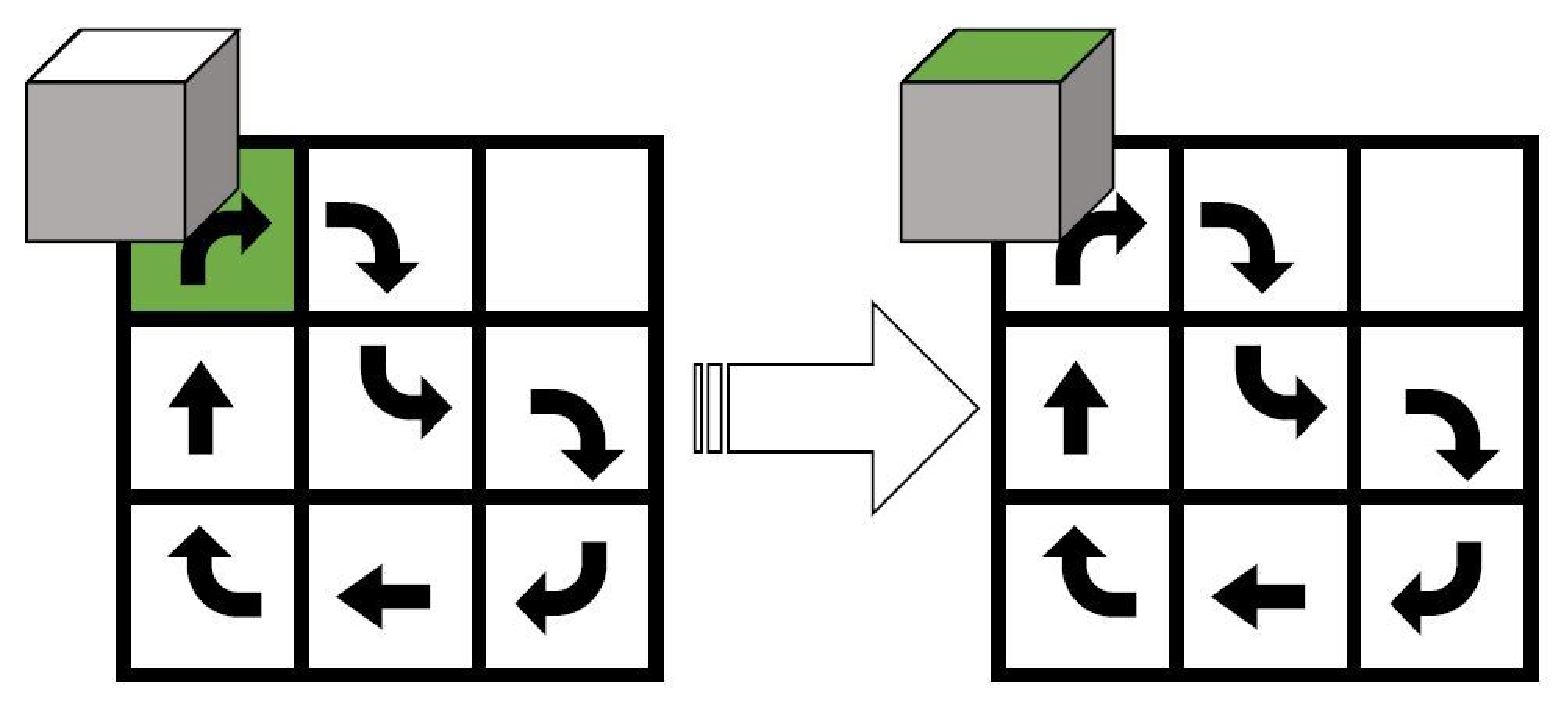
\includegraphics[width=0.5\textwidth]{Propuesta2secuencia4.pdf}
\caption{\emph{Captura} del cuadro activo dentro de la secuencia usando el dispositivo de control.}
\label{fig:Secuencia4}
\end{center}
\end{figure}

Una vez \emph{capturado}, se puede modificar los atributos (por ejemplo, el color), tocando sobre la pantalla (Figura ~\ref{fig:Secuencia5}), para después emplazarlo en otra localización de la secuencia (Figura ~\ref{fig:Secuencia6}).

\begin{figure}[!h]
\begin{center}
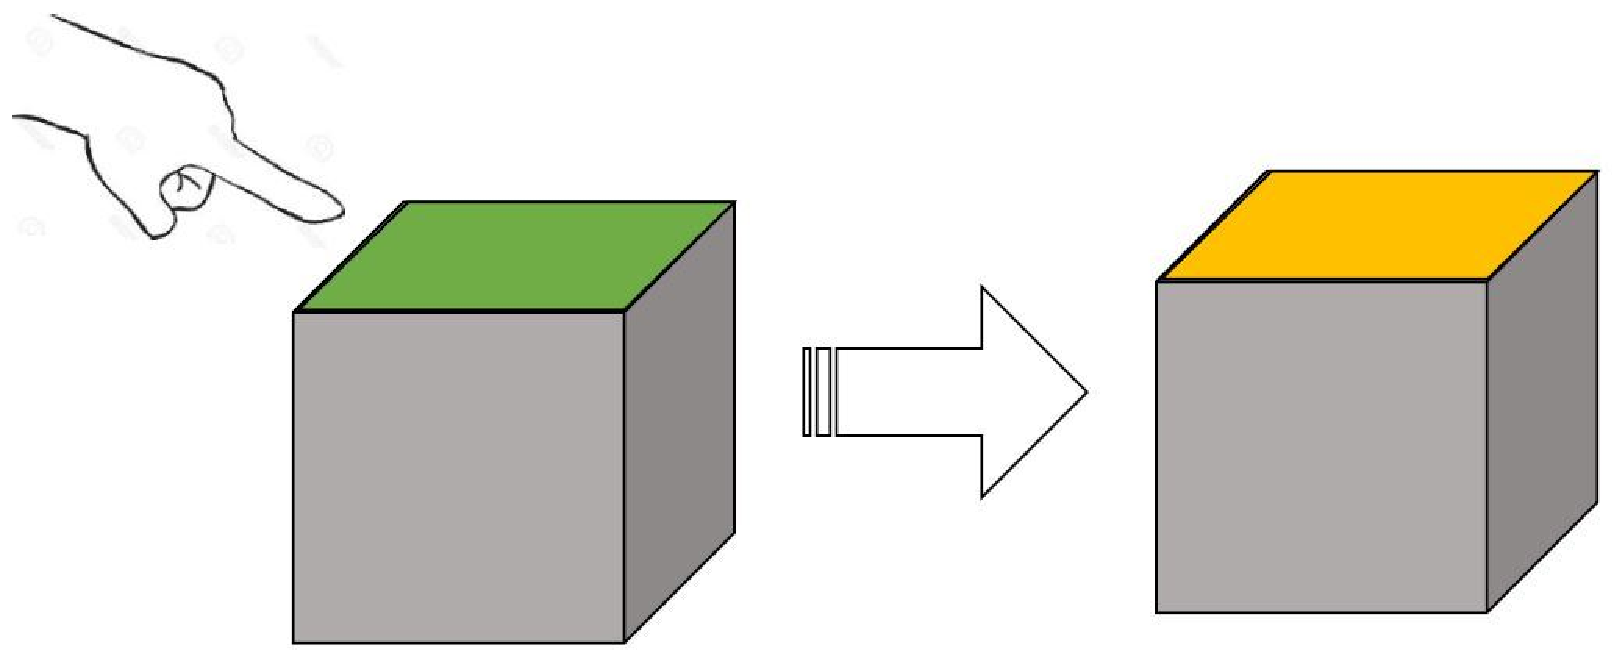
\includegraphics[width=0.5\textwidth]{Propuesta2secuencia5.pdf}
\caption{Modificación de la secuencia usando del dispositivo de control.}
\label{fig:Secuencia5}
\end{center}
\end{figure}

\begin{figure}[!h]
\begin{center}
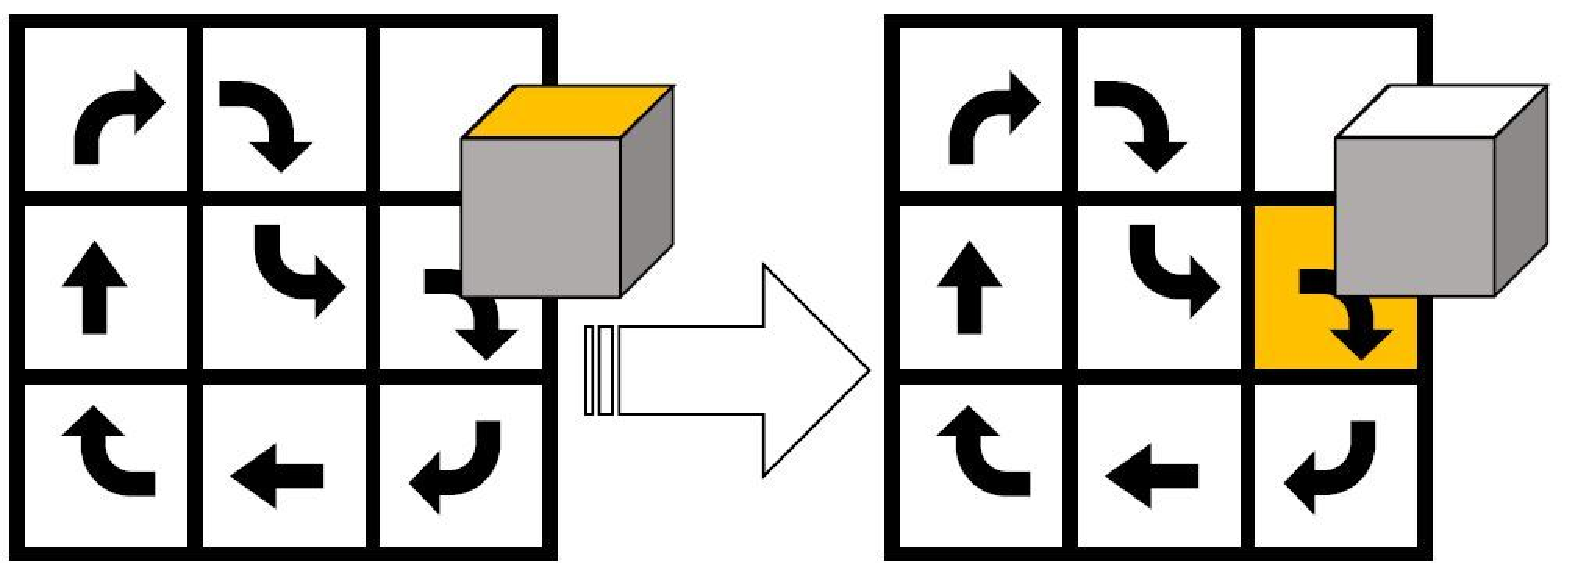
\includegraphics[width=0.5\textwidth]{Propuesta2secuencia6.pdf}
\caption{Emplazamiento dentro de la secuencia del cuadro modificado por medio del dispositivo de control.}
\label{fig:Secuencia6}
\end{center}
\end{figure}

\textbf{Análisis de la segunda propuesta de diseño}\\
La segunda propuesta de diseño es analizada junto con el director del proyecto. Se decide aceptar la propuesta al cubrir gran parte de las áreas de mejora localizadas en los actuales sistemas en la programación tangible. No obstante, se realizan algunas modificaciones, con el objetivo de eliminar posibles futuros problemas dentro del diseño e implementación.\\

\textbf{Posibles problemas y mejoras de la plataforma de juego.}\\
\begin{itemize}
\item Localización del dispositivo de control, sobre el dispositivo principal, usando un
magnetómetro. Debido a que el sensor no ofrece la precisión necesaria que requiere
la aplicación, para indicar la posición exacta de un dispositivo respecto a otro, se
decide eliminar este sistema de localización.
\item Definir un tamaño para ambos dispositivos que permita un correcto desarrollo de la interacción del juego.
\item Concretar la tecnología necesaria para implementar la aplicación en los dispositivos para un correcto funcionamiento.
\item Incorporar una unidad de medición inercial y sensores ópticos, que mejoren la experiencia de juego.
\end{itemize}


\subsubsection{Próximas historias de usuario.}
\begin{itemize}
\item Establecer requisitos iniciales.
\item Identificar y redactar objetivos.
\end{itemize}


\subsection{Iteración 4: Requisitos iniciales. Objetivos del TFG.}
\label{subs:itera4}
Establecer unos requisitos iniciales para empezar a desarrollar una plataforma de juego basada en interfaces tangibles, una vez se han analizado las posibilidades y limitaciones de las diferentes tecnologías actuales.\\
Los requisitos iniciales establecen las funcionalidades del dispositivo, y sirven de guía para el desarrollo del resto de la aplicación.\\
Los objetivos del proyecto son fijados a partir de la tecnología y requisitos iniciales obtenidos.\\ 
Los objetivos específicos podrán ser modificados durante el transcurso del resto de iteraciones, acorde con las necesidades del dispositivo.

\subsubsection{Requisitos iniciales del dispositivo.}
\textbf{Eliminar el uso de elementos externos al dispositivo.}\\
El uso de elementos externos para el funcionamiento del juego, como por ejemplo el uso de un teclado o una pantalla que el propio usuario debe disponer, en ocasiones puede acarrear un problema a la hora de utilizar el juego.
Para eliminar el uso de elementos externos para el funcionamiento del sistema de juego, se diseña un prototipo, el cual prescinda de dichos elementos, integrando todo lo necesario dentro de la misma plataforma.\\ 

\textbf{Reducir el elevado número de piezas para la interacción tangible.}\\
Un sistema de interacción tangible se caracteriza principalmente en que la información sea comprensible y literalmente captable, haciendo uso de objetos físicos que sean manipulables de forma natural. En ocasiones, el número de objetos físicos para el desarrollo del juego es elevado. Si bien es cierto que uno de los puntos más importantes a la hora de la programación para niños, es poder representar partes de código en diferentes elementos tangibles, un gran número de elementos puede suponer un problema para el niño a la hora del desarrollo del juego, pudiendo en algunos casos confundirlo.\\ 
Los sistemas de programación tangible utilizan bloques que al conectarlos o posicionarlos de una manera concreta, generan en tiempo real movimientos o acciones, bien mostrando la acción realizada en una pantalla, o bien mediante acciones llevadas a cabo por algún tipo de robot articulado, etc... Cada bloque indica una acción, por ejemplo, bloque de inicio, bloque de fin, bloque de dirección, bloque sensor...Para dar solución a este problema, la idea pasa por agrupar los bloques tangibles, que son utilizados en la interacción del juego y que tienen como finalidad representar una acción, en un solo elemento tangible. Se propone el diseño de un dispositivo tangible que, por medio de un microprocesador, muestre en una pantalla estas funciones.

\textbf{Ampliar el enfoque del rango de edades en el juego. Diseño dinámico del juego.}\\
La mayoría de los diseños actuales de dispositivos dedicados a la programación tangible, están enfocados a un rango de edades determinado. Un juego puede resultar demasiado simple o demasiado complejo para algunos niños, debido a la edad de estos. Otro punto que tener en consideración, es el diseño estático en los juegos. El usuario dispone de unos recursos para ser utilizados, y aunque las combinaciones y posiciones de elementos tangibles permiten realizar diferentes acciones de juego, no dejan de ser siempre los mismos elementos con los mismos propósitos. Estos dos puntos están relacionados con una característica común, no tienen la posibilidad de mejorar, no pueden ser actualizados, al menos que se adquiera una nueva versión del producto, lo que perjudica al usuario final.

\textbf{Reducir costes de los bloques o dispositivos de realimentación.}\\
El alto coste de los bloques o dispositivos de realimentación, al igual que el uso de un gran número de elementos empleados en la interacción tangible, eleva el precio del diseño.\\



\textbf{Requisitos iniciales del dispositivo, a partir de las áreas de mejoras localizadas en los diferentes aplicaciones dedicadas a la programación tangible para niños:}\\
\begin{itemize}
\item Dispositivo completo e independiente de elementos externos al mismo.
\item Agrupar elementos tangibles en un solo dispositivo tangible.
\item Disponer de actualizaciones software, para mejoras la plataforma.
\item Utilización de elementos de bajo coste para el diseño.
\end{itemize}



\textbf{Requisitos de diseño del juego dentro de la plataforma:}
\begin{itemize}
\item Fácil de entender.
\item Apropiado para realizar el juego de forma libre.
\item Bloques simples que representen el vocabulario/léxico.
\item Posibilidad de realizar un gran número de programas.
\item Mejorar/depurar sin necesidad de herramientas externas.
\end{itemize}

\subsubsection{Objetivos del TFG}

\textbf{Objetivo general}: Diseñar y desarrollar una plataforma interactiva de juego de bajo coste, basada en interfaces tangibles, haciendo uso de las nuevas tecnologías, para promover el desarrollo de capacidades en niños de corta edad.

\textbf{Objetivos específicos}:
\begin{itemize}
\item Diseñar y programar un sistema de localización y reconocimiento de las interfaces de usuario tangibles.

\item Desarrollar un sistema eficiente de transferencia de datos entre ambas interfaces tangibles.

\item Realizar una correcta sincronización en la visualización de la aplicación entre ambas pantallas, que permita una buena representación de juego.

\item Ofrecer un entorno gráfico simple, que permita al niño ser capaz de diseñar secuencias y modificarlas, por medio de elementos tangibles.

\item Adaptar sensores inerciales y ópticos para una mejor experiencia de juego, donde ambos elementos tangibles interactúen entre sí, permitiendo la manipulación de la información entre los dispositivos.

\item Diseñar un sistema de actualización de software de los dispositivos, a través de la conexión externa a un servidor.
\end{itemize}


\subsubsection{Próximas historias de usuario.}
\begin{itemize}
\item Tecnologías para el desarrollo.
\item Diseño de la plataforma de juego, a partir de los requisitos y objetivos fijados.
\end{itemize}



\subsection{Iteración 5: Diseño de la plataforma de juego. Tecnologías para el desarrollo. }

\subsubsection{Descripción de la plataforma de juego propuesta en el proyecto.}
Este diseño pretende abordar los problemas señalados en la iteración 4 \ref{subs:itera4} de este documento, introduciendo \emph{TUIOs}\footnote{Tangible User Interface Objects} accionados que son controlables por el sistema, con el fin de representar cambios dinámicos de la información, combinando elementos tangibles, gráficos y nuevas tecnologías. La plataforma de juego se basa en los conceptos de secuenciación, repetición de bucles, y programación creativa.

La idea principal parte de que los niños no sean simplemente consumidores de contenido y que tengan la posibilidad de crearlo, que ellos mismos sean capaces de tomar decisiones durante el juego de una manera tangible e intuitiva. El sistema de juego abarca desde el desarrollo de una secuencia a partir de los criterios de creación del niño, hasta la resolución de pequeños problemas de lógica.

La plataforma ofrece un entorno de juego compartido entre dos dispositivos tangibles principales, \emph{TUIO1} y \emph{TUIO2}. Ambos dispositivos disponen de interfaz gráfica con panel táctil, para la visualización y desarrollo del juego. Los eventos durante el juego son transmitidos vía inalámbrica. La plataforma incorpora sensores para mejorar la experiencia de juego. 
 
A continuación, son detallados los componentes y características de cada dispositivo.


\textbf{Dispositivo TUIO1.}\\
Este dispositivo integra un ordenador de placa reducida \emph{Raspberry Pi}, que maneja todos los eventos generados durante el juego. Se encarga de la representación gráfica principal del juego por medio de una pantalla de 7 pulgadas táctil capacitiva (ver Figura ~\ref{fig:TUIO1}). Otra de las características es que dispone de una salida de audio para eventos tipo acústicos.

\begin{figure}[!h]
\begin{center}
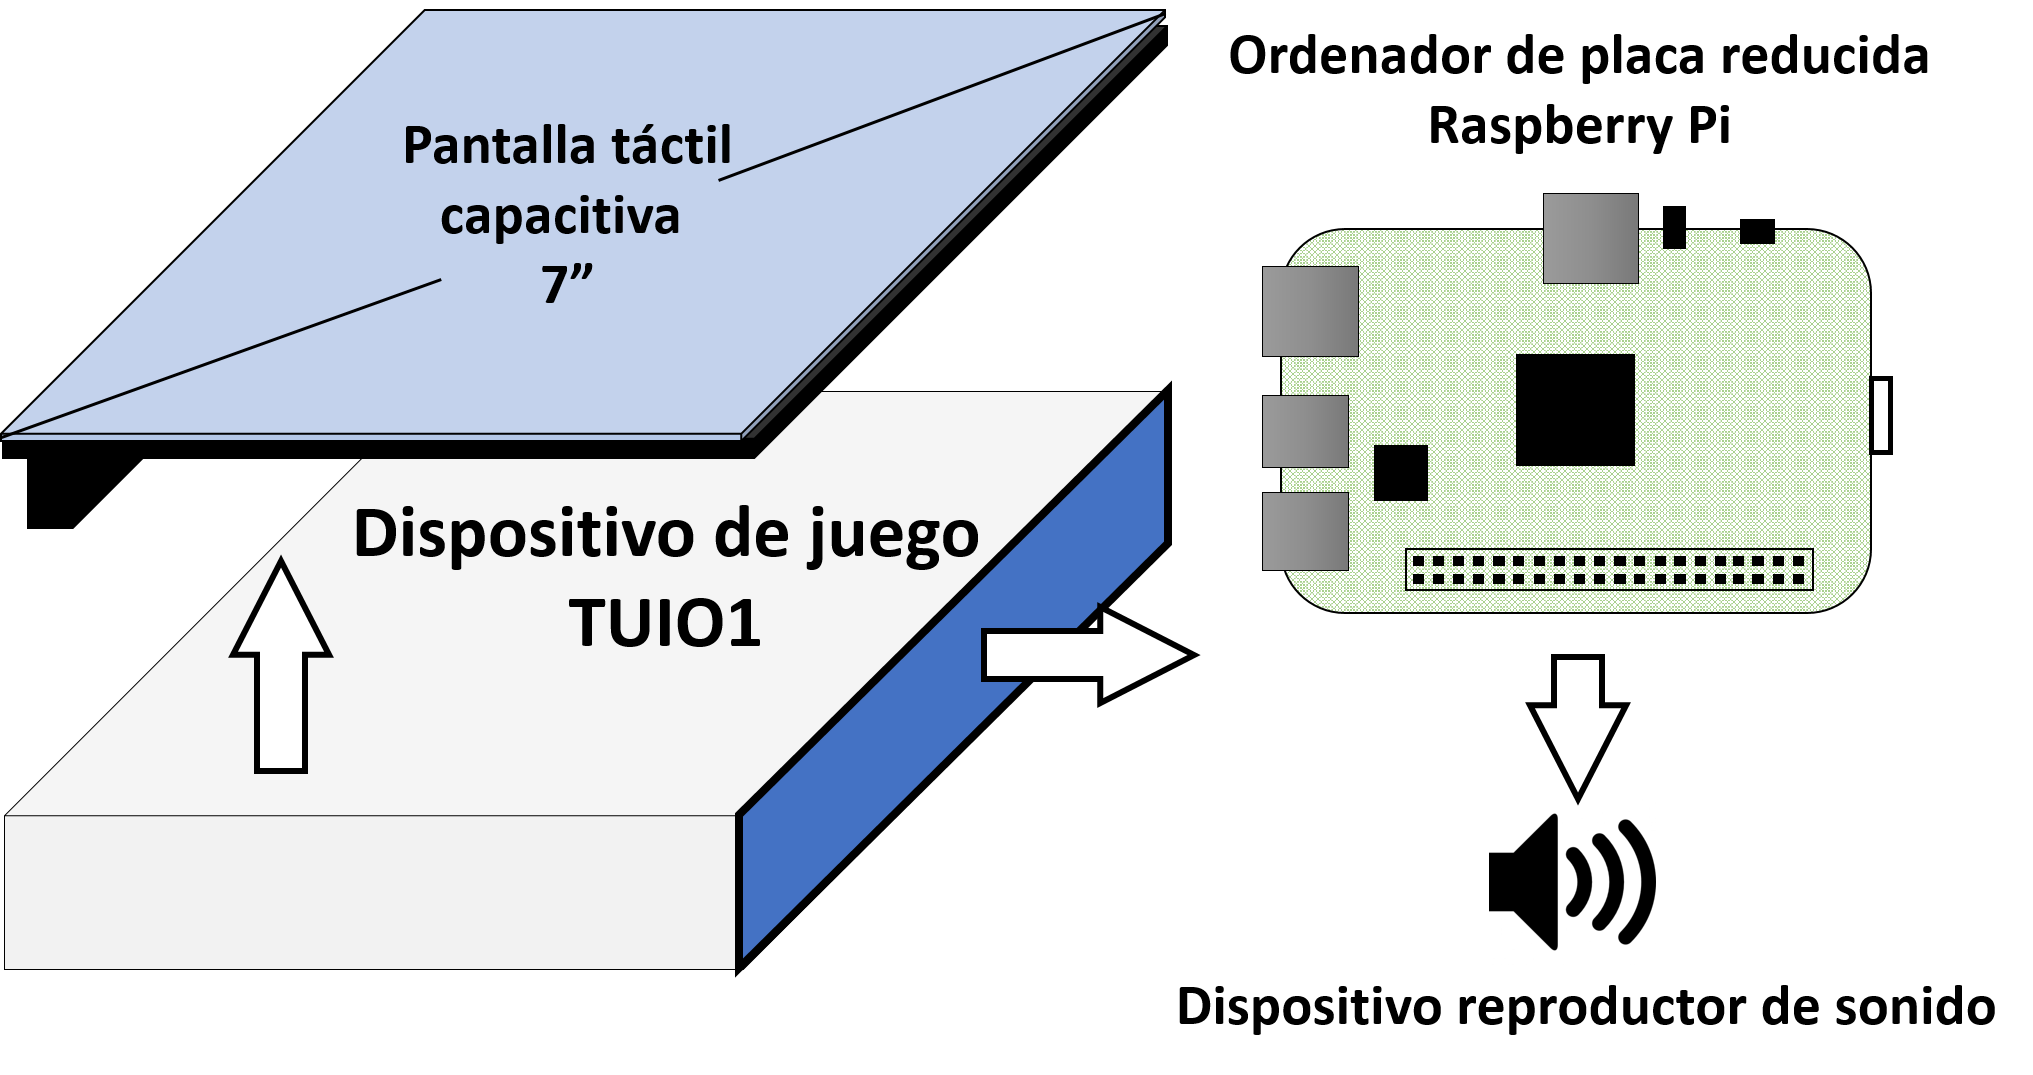
\includegraphics[width=0.8\textwidth]{TUIO1.png}
\caption{Dispositivo de juego TUIO1.}
\label{fig:TUIO1}
\end{center}
\end{figure}


\textbf{Placa para el desarrollo en TUIO1. Raspberry Pi.}\\
Esta placa dispone de un microprocesador \emph{BCM2837} de 64 bits de cuádruple núcleo a 1,2GHz, 1GB de memoria \emph{RAM} y \emph{GPU} de doble núcleo Videocore IV, que permite manejar y procesar eventos e imágenes según los requisitos de la aplicación.
Integra el chip \emph{BCM43143} para la comunicación \emph{WiFi} entre dispositivos, lo que elimina la necesidad de utilizar cables. Interfaz gráfica de usuario por puerto HDMI.
Incorpora 40 pines \emph{GPIO}, los cuales disponen de un bus \emph{I2C} \footnote{I2C, «Inter-Integrated Circuit».} para la utilización de sensores dentro del sistema de juego, y un bus \emph{SPI}\footnote{SPI, «Serial Peripheral Interface» } como alternativa al puerto HDMI para mostrar la interfaz gráfica de usuario.
Su reducido tamaño, bajo consumo, además de contar con una gran comunidad de usuarios, hacen de este dispositivo el adecuado para la realización de un prototipo de plataforma de juego.\\


La documentación relacionada con este dispositivo, se encuentra detallada en: \emph{Sección ~\ref{subsubs:rasp} Raspberry Pi 3B.}

Toda la documentación relacionada con el dispositivo \emph{Raspberry Pi}, se encuentra detallada en el Capítulo 5 Tecnologías para el desarrollo. Hardware y Software, en la sección 5.1.1 Raspberry Pi 3.

\textbf{Elementos para la representación intangible de la información en TUIO1}.\\
Si bien los elementos tangibles juegan el papel central en la representación y control en una interfaz de usuario tangible, la representación intangible es también importante, siendo esta información dinámica proporcionada, una gran ayuda al realizar una interacción. La existencia en tiempo real de una realimentación de la representación intangible, cuando se ha manipulado la representación tangible, es fundamental para asegurar un correcto acoplamiento perceptivo. Las representaciones intangibles que incorpora el diseño son auditivas y gráficas. Estas representaciones se producen en determinados momentos en desarrollo del juego.

\textbf{Interfaz gráfica en \emph{TUIO1}.}\\
Pantalla táctil capacitiva de 7 pulgadas para la representación gráfica del juego. Una pantalla capacitiva detecta varias pulsaciones simultaneas sobre ella. Esta característica es fundamental para desarrollar un sistema de localización del dispositivo \emph{TUIO2} sobre la pantalla.
La conexión de la interfaz gráfica con la placa para el desarrollo es HDMI, por su compatibilidad y facilidad de uso con \emph{Raspberry Pi}. Los eventos generados en el panel táctil son transmitidos desde el puerto \emph{Micro USB-B}, al puerto de comunicaciones \emph{USB-A} de la placa. La Figura ~\ref{fig:Conexion_Pantalla} muestra las conexiones de ambas interfaces.
Se considera que las dimensiones de la pantalla son las adecuadas para una correcta visualización de los contenidos del juego. Queda abierta la posibilidad del empleo de una pantalla de mayores dimensiones.

\begin{figure}[!h]
\begin{center}
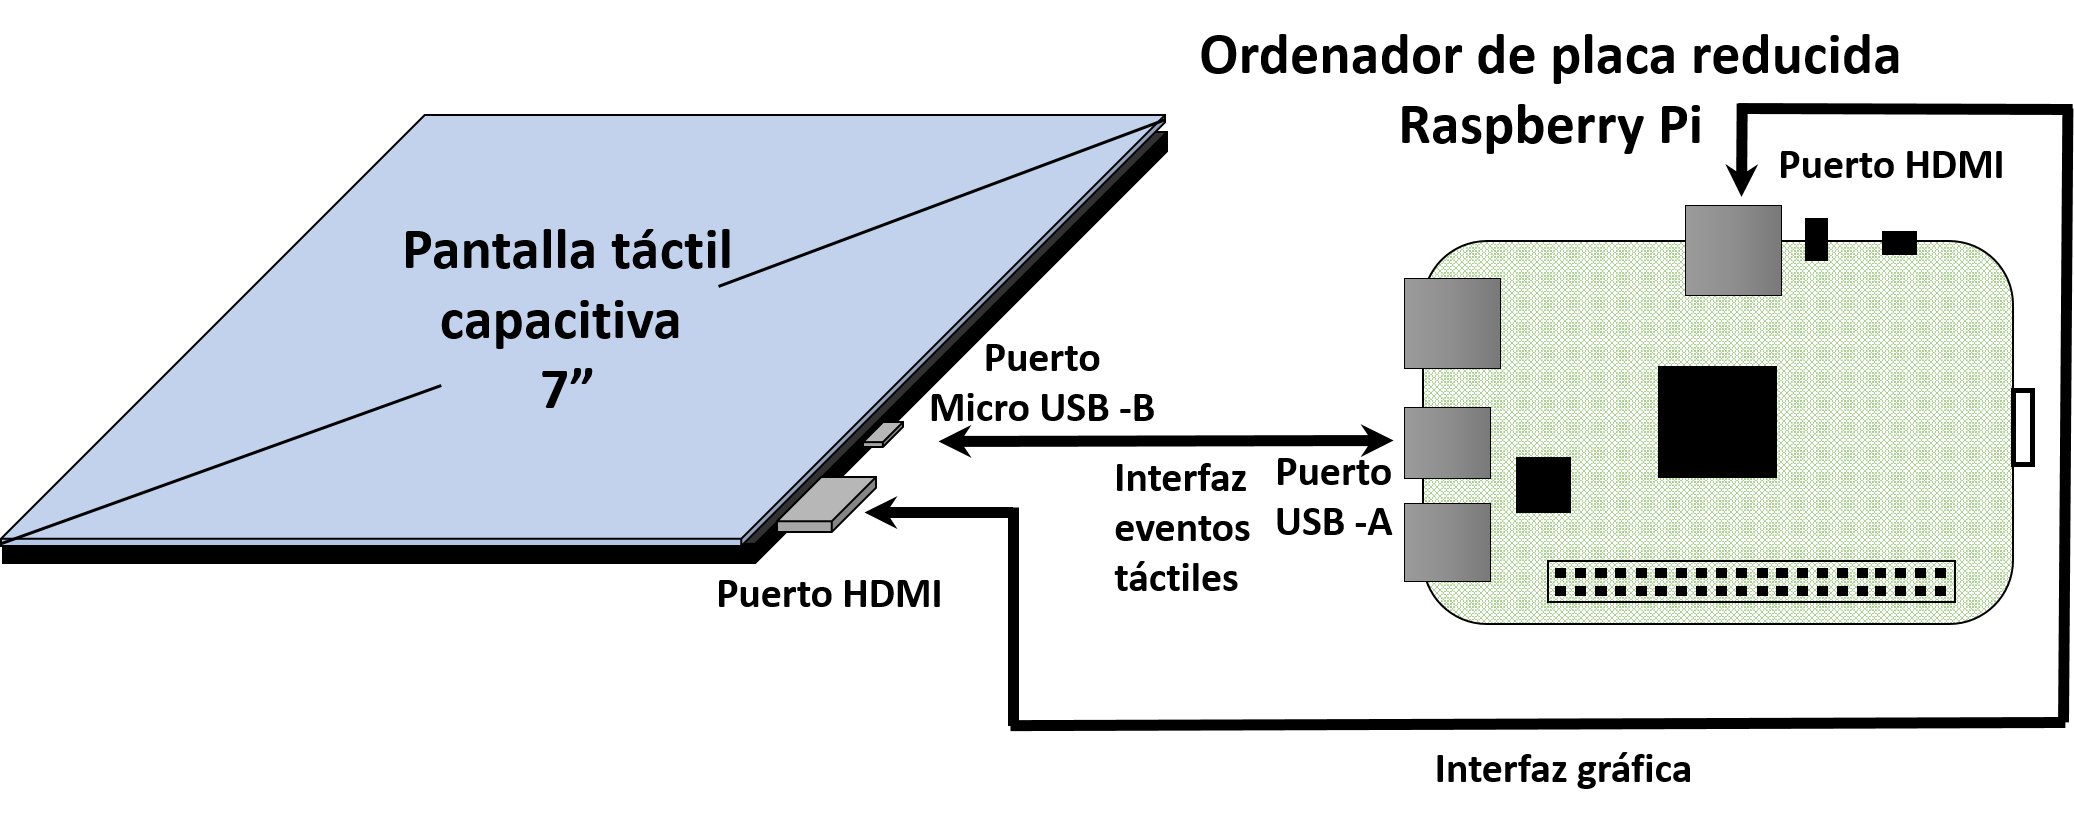
\includegraphics[width=0.8\textwidth]{Conexion_Pantalla.png}
\caption{Conexión de la interfaz gráfica de usuario y interfaz de eventos táctiles, entre pantalla y Raspberry Pi.}
\label{fig:Conexion_Pantalla}
\end{center}
\end{figure}

La documentación relacionada con este dispositivo, se encuentra detallada en: \emph{Sección ~\ref{subsubs:pantalla7} Pantalla táctil capacitiva HDMI.}

\textbf{Dispositivo \emph{TUIO2}.}\\
Este dispositivo está diseñado con la finalidad de agrupar las acciones, movimientos, apariencia, eventos acústicos, parámetros, etc., que definen un lenguaje de programación tangible. Esta agrupación elimina el problema de disponer de distintos elementos tangibles para el desarrollo del juego. \emph{TUIO2} hace de puente entre la interfaz física y la digital.
La idea es mostrar de forma gráfica en una pantalla de 3,5 pulgadas, todos estos elementos de programación para crear una secuencia, y ser aplicados al juego por medio una interacción física (sistema de localización), o transmitir estas instrucciones de forma inalámbrica. El sistema de localización aplicado en la interacción física es posible gracias a unas almohadillas conductivas situadas en la parte posterior del dispositivo, y que son detectadas por la pantalla capacitiva de \emph{TUIO1}.
\emph{TUIO2} dispone de dos sensores. Un sensor de color, y una unidad de medición inercial. Estos sensores son utilizados para mejor la experiencia de juego.
La Figura ~\ref{fig:TUIO2} muestra una representación general del dispositivo \emph{TUIO2}.

\begin{figure}[!h]
\begin{center}
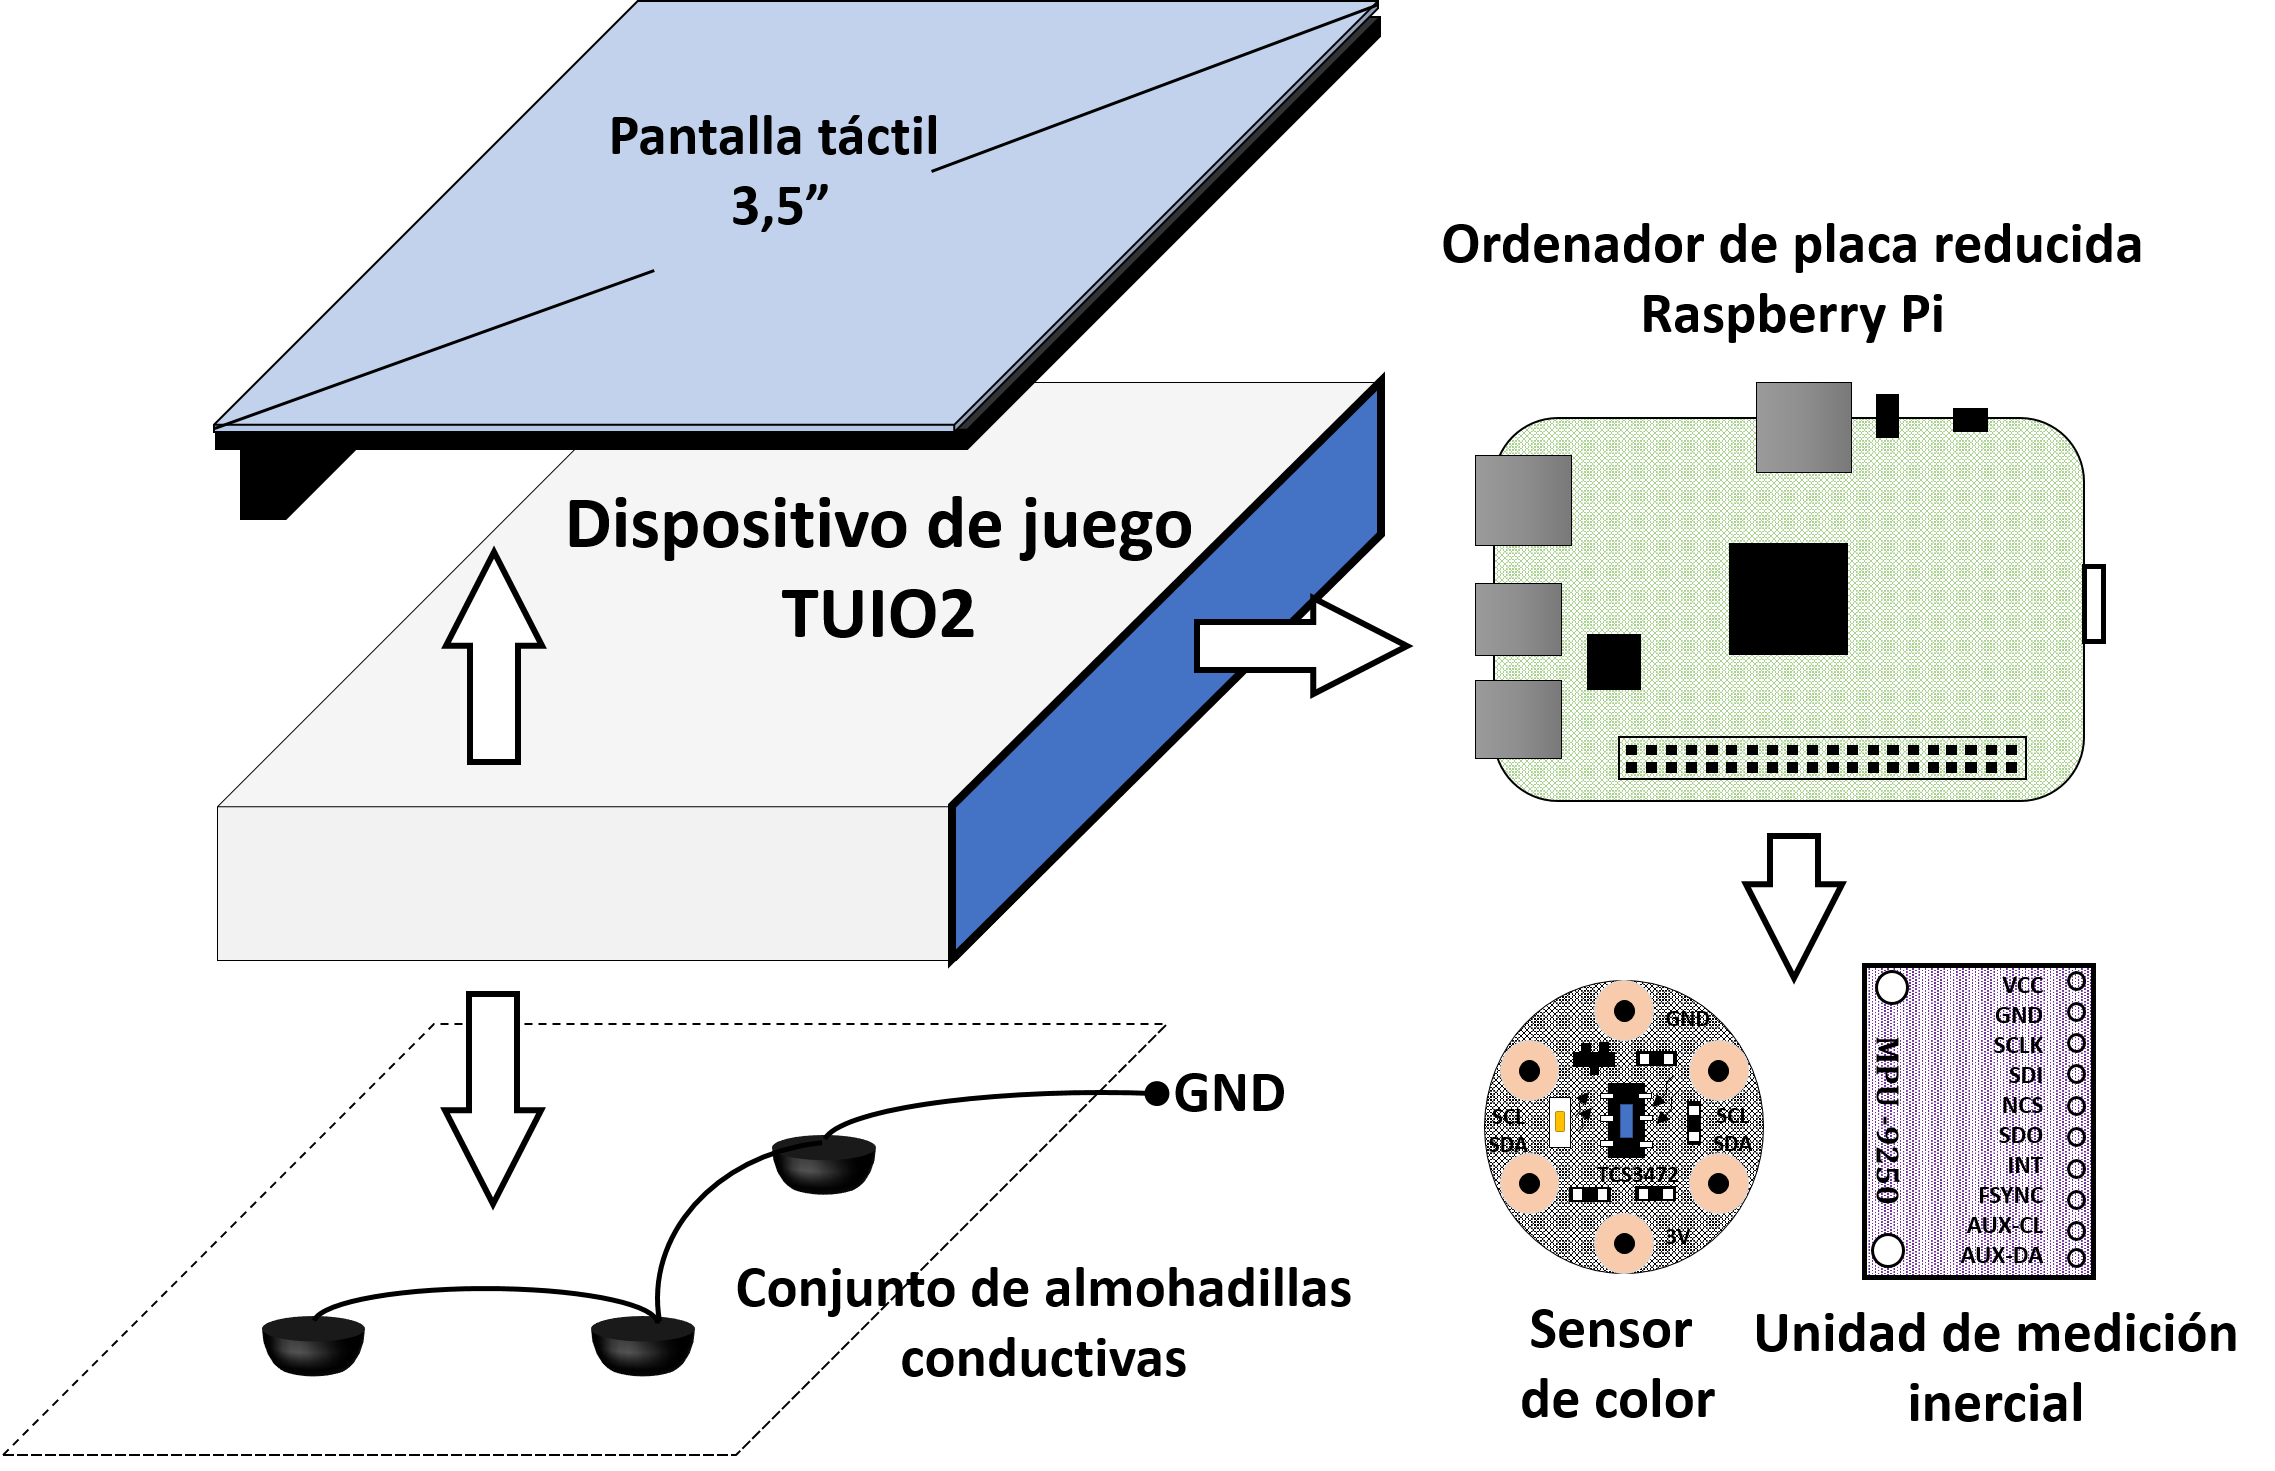
\includegraphics[width=0.8\textwidth]{TUIO2.png}
\caption{Dispositivo de juego TUIO2.}
\label{fig:TUIO2}
\end{center}
\end{figure}


\textbf{Placa para el desarrollo en \emph{TUIO2}.}\\
Al igual que \emph{TUIO1}, este dispositivo integra un ordenador de placa reducida \emph{Raspberry Pi}, que maneja todos los eventos generados durante el juego.


\textbf{Sistema de localización de TUIO2 sobre TUIO1.}\\
Un panel táctil de tipo capacitivo detecta varios eventos sobre el mismo, por lo general un dedo un humano, pero también detecta la presencia de un conductor eléctrico conectado a tierra. Estas dos características ofrecen la posibilidad de detectar la posición del dispositivo \emph{TUIO2} sobre \emph{TUIO1}.
Por ejemplo, si se desea ordenar al juego realizar un desplazamiento hacia la derecha dentro de la secuencia, el dispositivo \emph{TUIO2} muestra de forma gráfica esta acción (símbolo hacia la derecha), y puede realizar esta instrucción simplemente presionando sobre el símbolo, o posicionar el dispositivo sobre la pantalla de \emph{TUIO1}. El dispositivo \emph{TUIO2} dispone de unas almohadillas conductivas (ver Figura ~\ref{fig:Almohadillas_tuio2}) que son detectadas por la pantalla de \emph{TUIO1}. Esto es posible debido a la capacidad de detectar varios eventos táctiles de una pantalla capacitiva. La pantalla de \emph{TUIO1} refleja dentro de la secuencia la instrucción enviada.  


\begin{figure}[!h]
\begin{center}
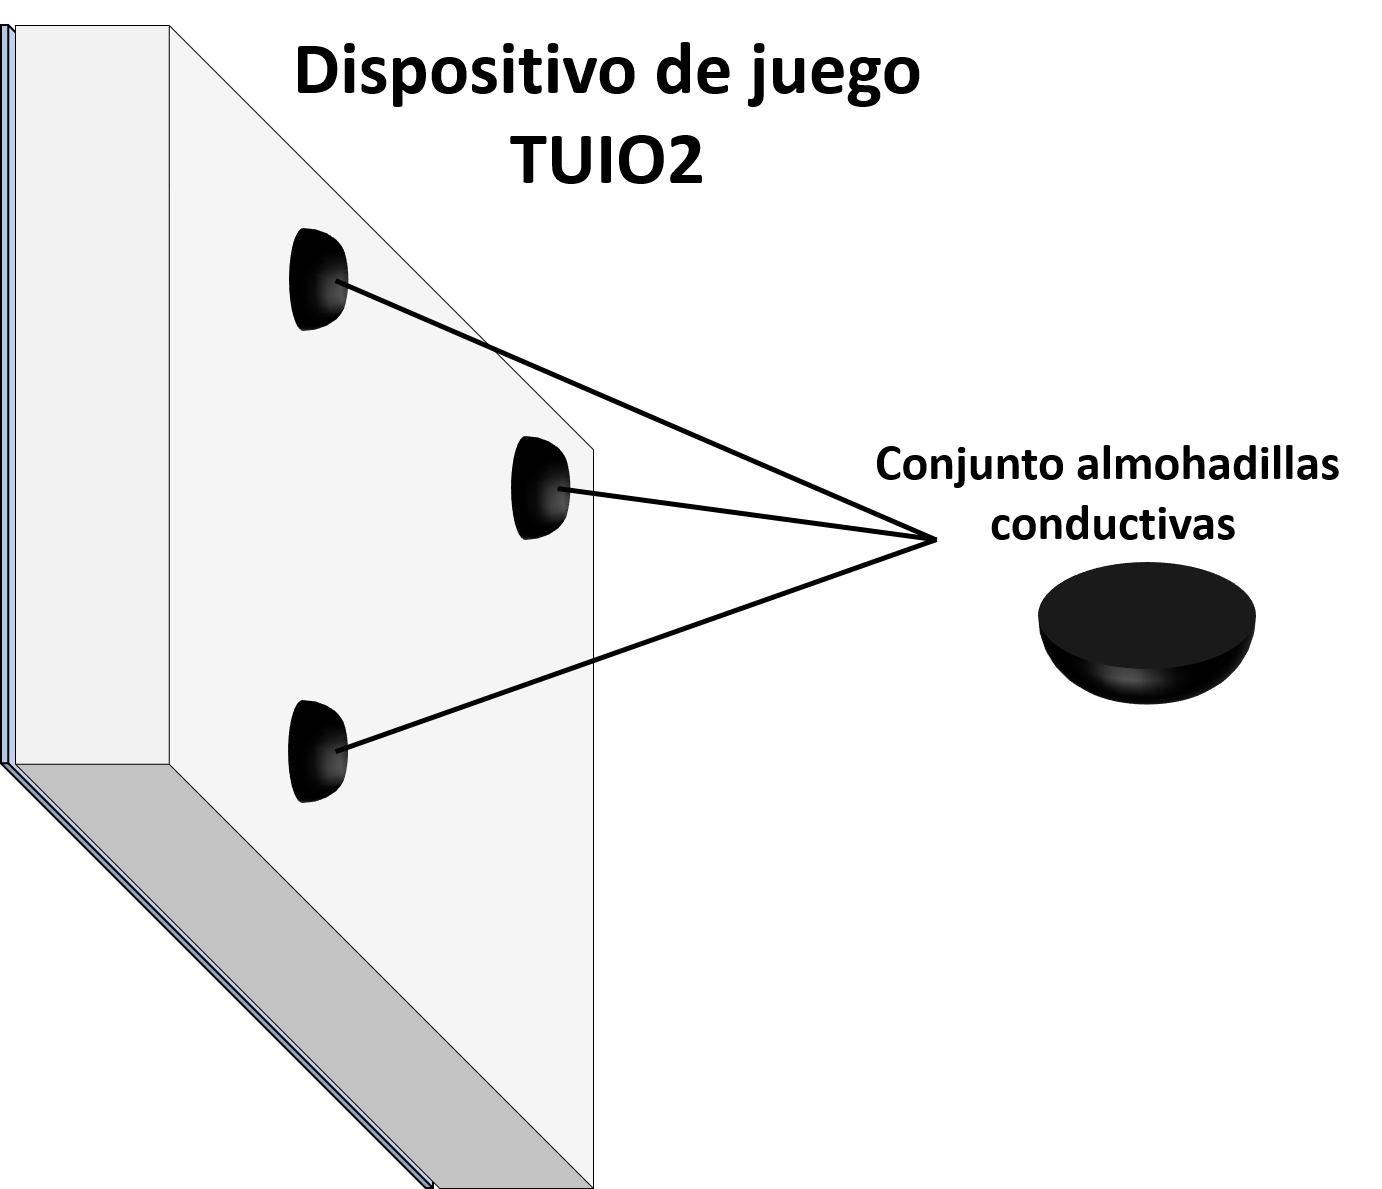
\includegraphics[width=0.8\textwidth]{Almohadillas_tuio2.png}
\caption{Disposición de las almohadillas conductivas en dispositivo de juego TUIO2.}
\label{fig:Almohadillas_tuio2}
\end{center}
\end{figure}

\textbf{Interfaz gráfica en \emph{TUIO2}.}\\
Pantalla táctil resistiva de 3.5 pulgadas para la representación gráfica del juego.
La conexión de la interfaz gráfica con la placa para el desarrollo es \emph{HDMI}, por su compatibilidad y facilidad de uso con Raspberry Pi. Los eventos generados en el panel táctil son transmitidos a la placa por comunicación \emph{SPI}. La Figura ~\ref{fig:Conexion_Pantalla2} muestra las conexiones de ambas interfaces.
Se considera que las dimensiones de la pantalla son las adecuadas para una correcta visualización de los contenidos del juego. Queda abierta la posibilidad del empleo de una pantalla de mayores dimensiones.

\begin{figure}[!h]
\begin{center}
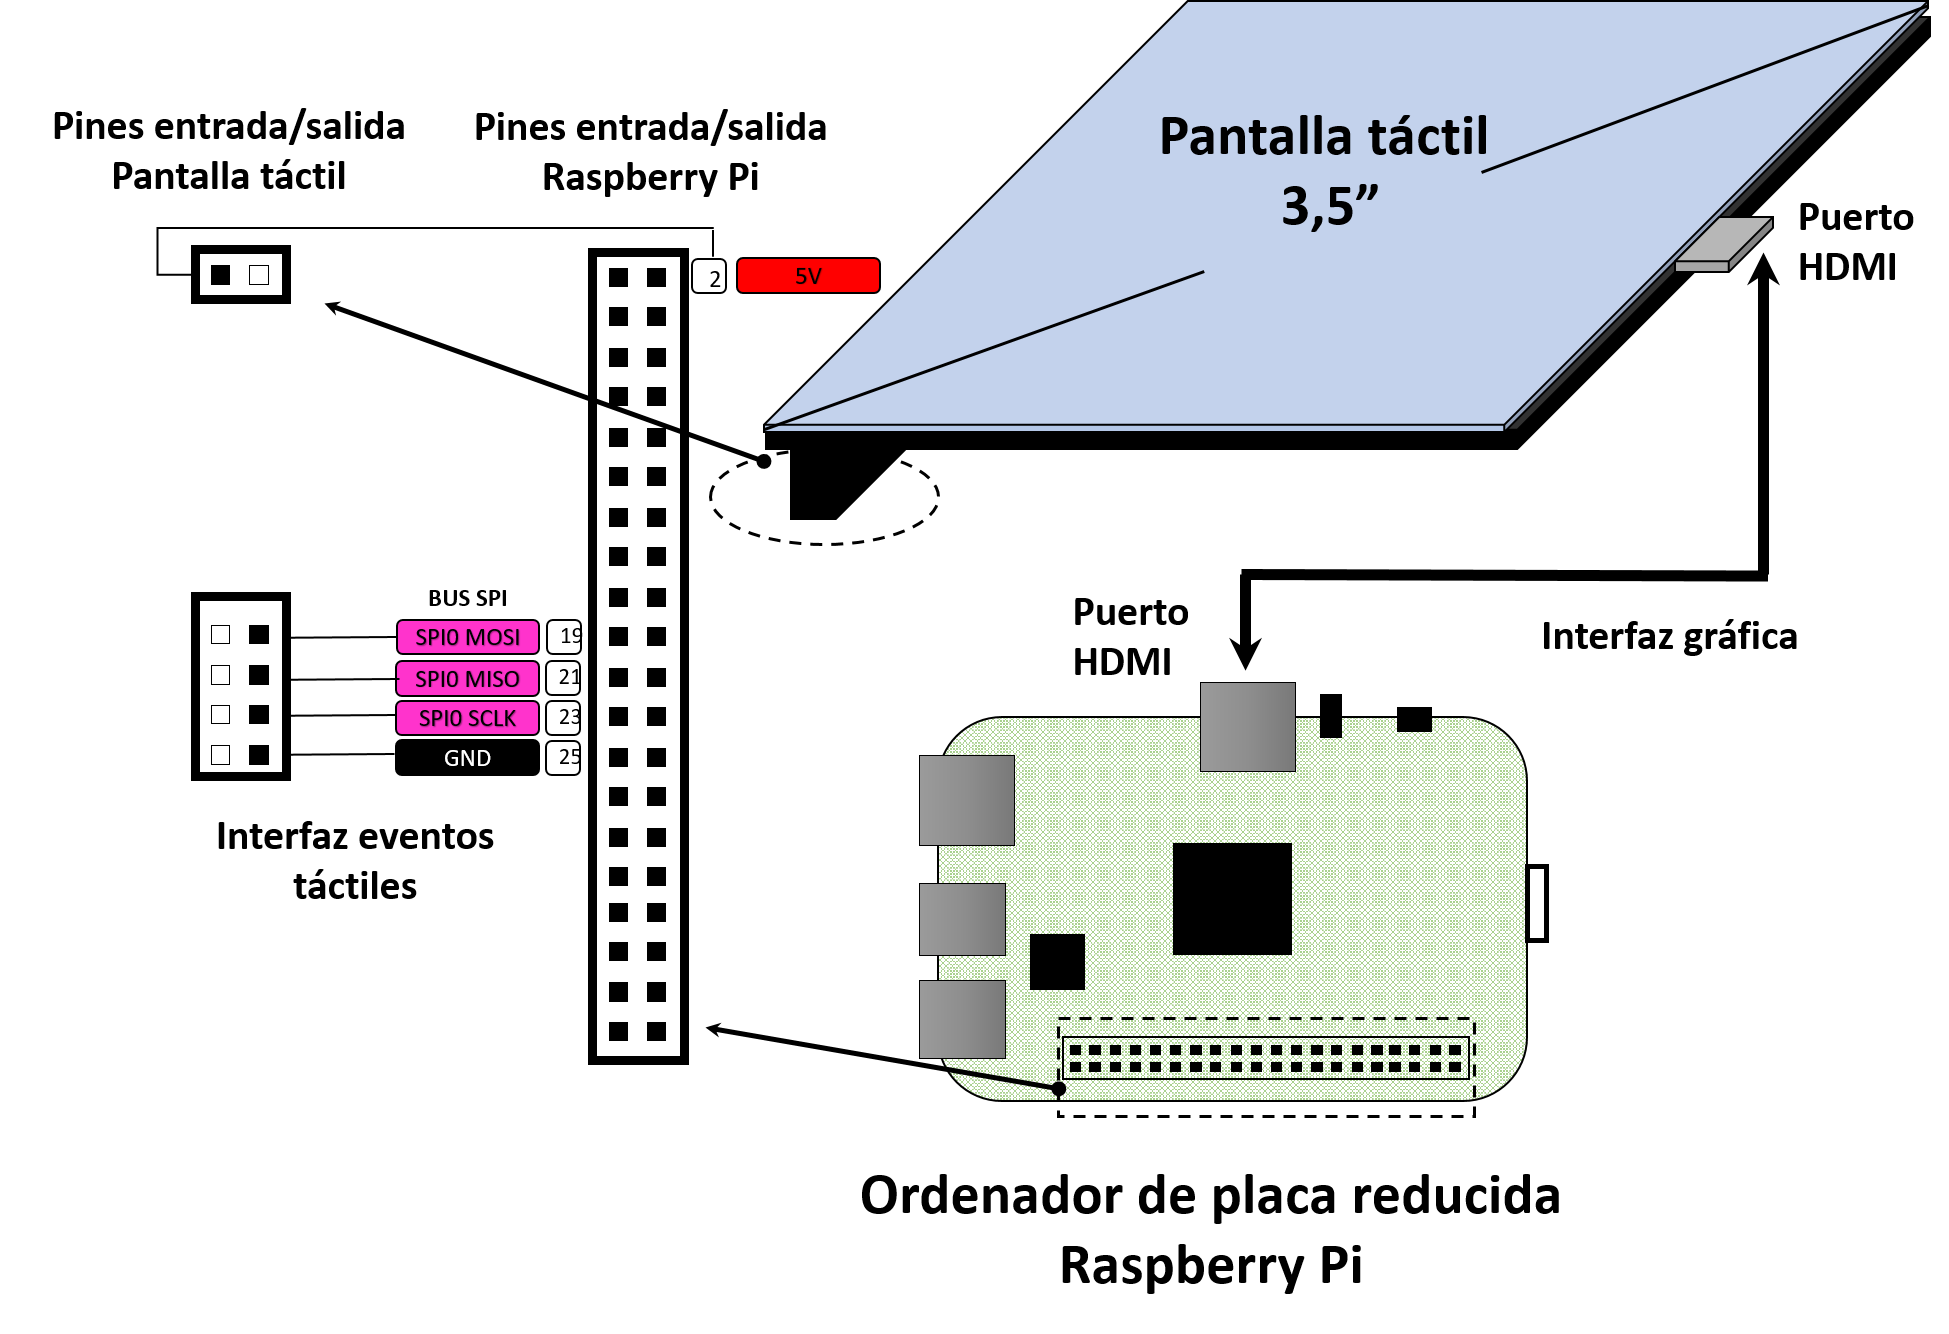
\includegraphics[width=0.8\textwidth]{Conexion_Pantalla2.png}
\caption{Conexión de la interfaz gráfica de usuario y interfaz de eventos táctiles, entre pantalla y Raspberry Pi en TUIO2.}
\label{fig:Conexion_Pantalla2}
\end{center}
\end{figure}

La documentación relacionada con este dispositivo, se encuentra detallada en: \emph{Sección ~\ref{subsubs:pantalla3} Pantalla táctil resistiva HDMI.}

\textbf{Sensores implementados en el dispositivo TUIO2.}\\

Uno de los objetivos específicos es adaptar sensores inerciales y ópticos para una mejor experiencia de juego, donde los elementos \emph{TUIO1} y \emph{TUIO2} interactúen entre sí, permitiendo la manipulación de la información entre los dispositivos.

\textbf{Unidad de medición inercial.}\\
La unidad de medición inercial integrada en la plataforma, es el sensor \emph{MPU9255}. Este sensor forma parte del dispositivo \emph{TUIO2}. Esta destinado principalmente a capturar eventos de movimiento, para generar acciones durante el transcurso del juego. Al realizar movimientos angulares sobre los ejes X,Y,Z del dispositivo \emph{TUIO2}, se generan unos eventos que son filtrados y comunicados al dispositivo \emph{TUIO1}, para ser ejecutados durante el transcurso del juego. Por ejemplo, girar una pieza representada en \emph{TUIO1} (Ver Figura ~\ref{fig:IMU_TUIO2}).

\begin{figure}[!h]
\begin{center}
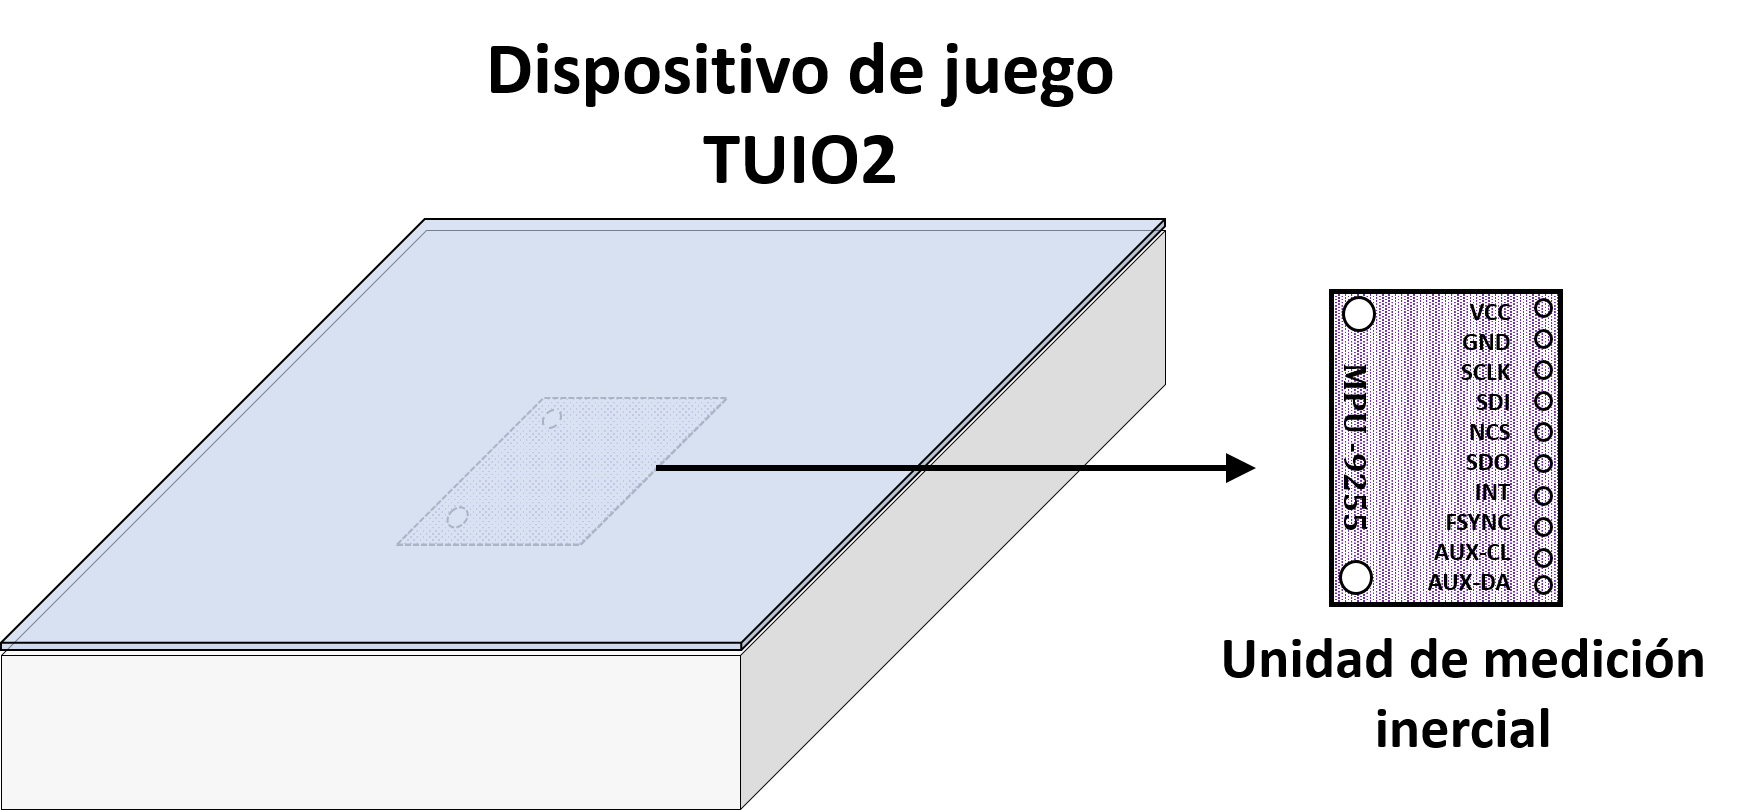
\includegraphics[width=0.8\textwidth]{IMU_TUIO2.png}
\caption{Ejemplo de aplicación de desplazamientos angulares mediante la unidad de medición inercial.}
\label{fig:IMU_TUIO2}
\end{center}
\end{figure}


\textbf{Sensor de color.}\\
Los sensores de color detectan el color de una superficie, y entregan la información de manera digital.
El dispositivo implementado es el sensor de color \emph{TCS34725}, que proporciona un retorno digital de los valores de detección de luz roja, verde y azul (RGB). Dispone de un filtro de bloqueo \emph{IR}\footnote{Infrared radiation} para una mejor detección de la luz ambiente.\
La integración de este dispositivo (ver Figura ~\ref{fig:TUIO2_ColorSensor}), hace posible una interacción directa con el medio que le rodea, lo que permite ampliar las opciones de juego dentro de la plataforma. Por ejemplo, localizar objetos de color rojo. La información de color obtenida sirve para cambiar parámetros, o generar eventos durante el transcurso del juego (ver Figura ~\ref{fig:TUIO_Color1}).

\begin{figure}[!h]
\begin{center}
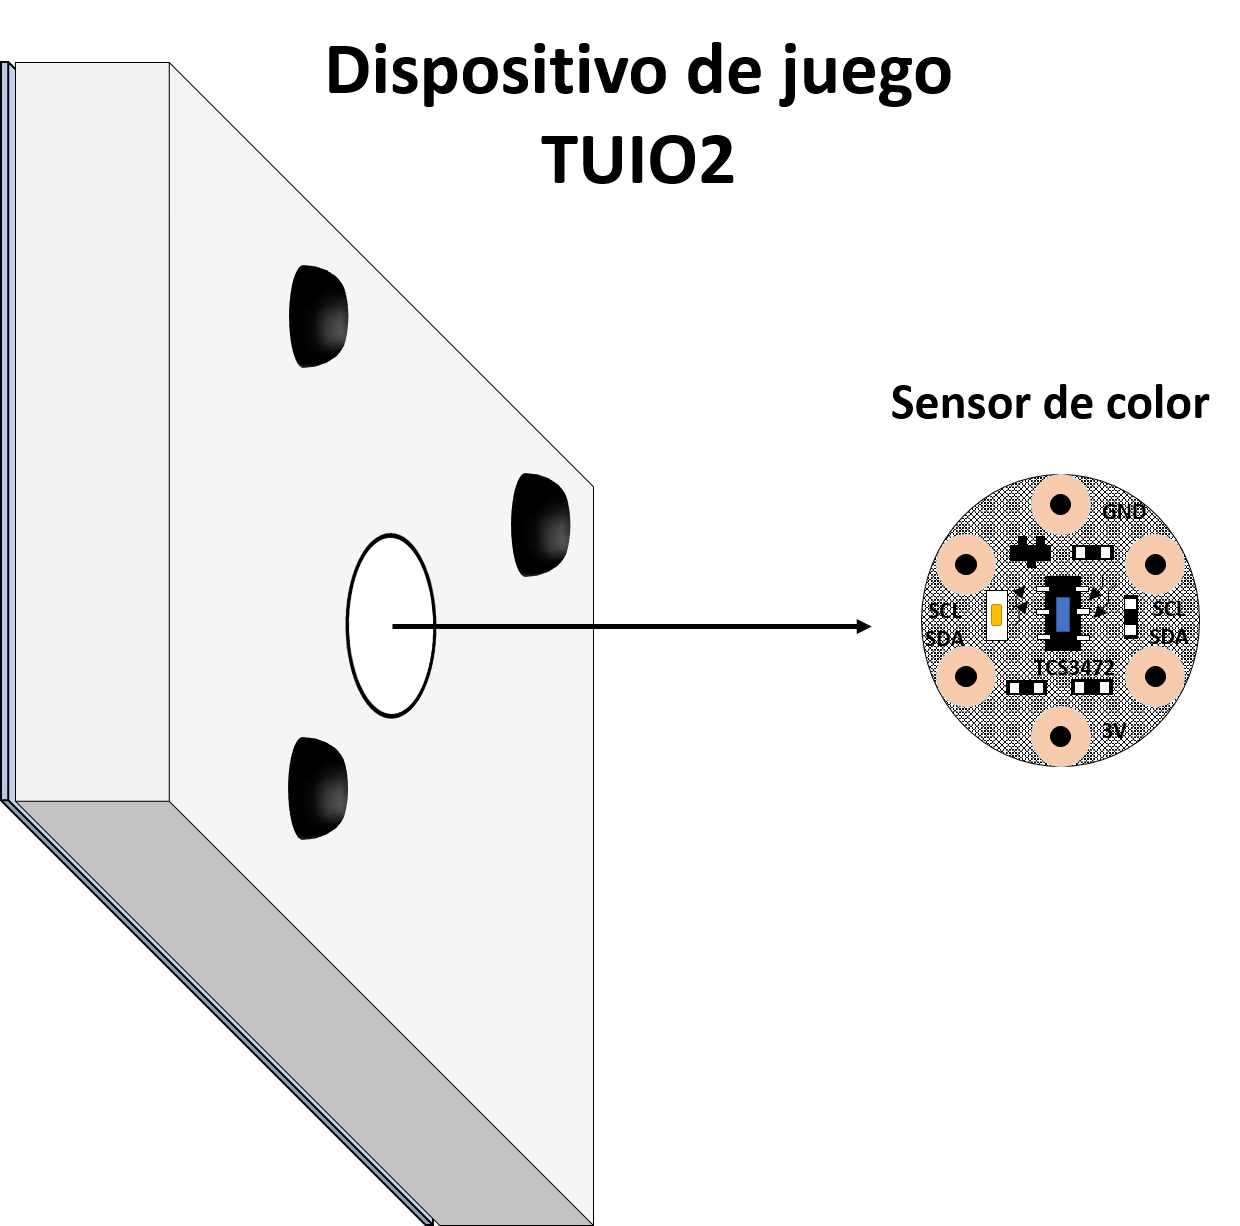
\includegraphics[width=0.7\textwidth]{TUIO2_ColorSensor.png}
\caption{Sensor de color incorporado en el dispositivo TUIO2.}
\label{fig:TUIO2_ColorSensor}
\end{center}
\end{figure}


\begin{figure}[!h]
\begin{center}
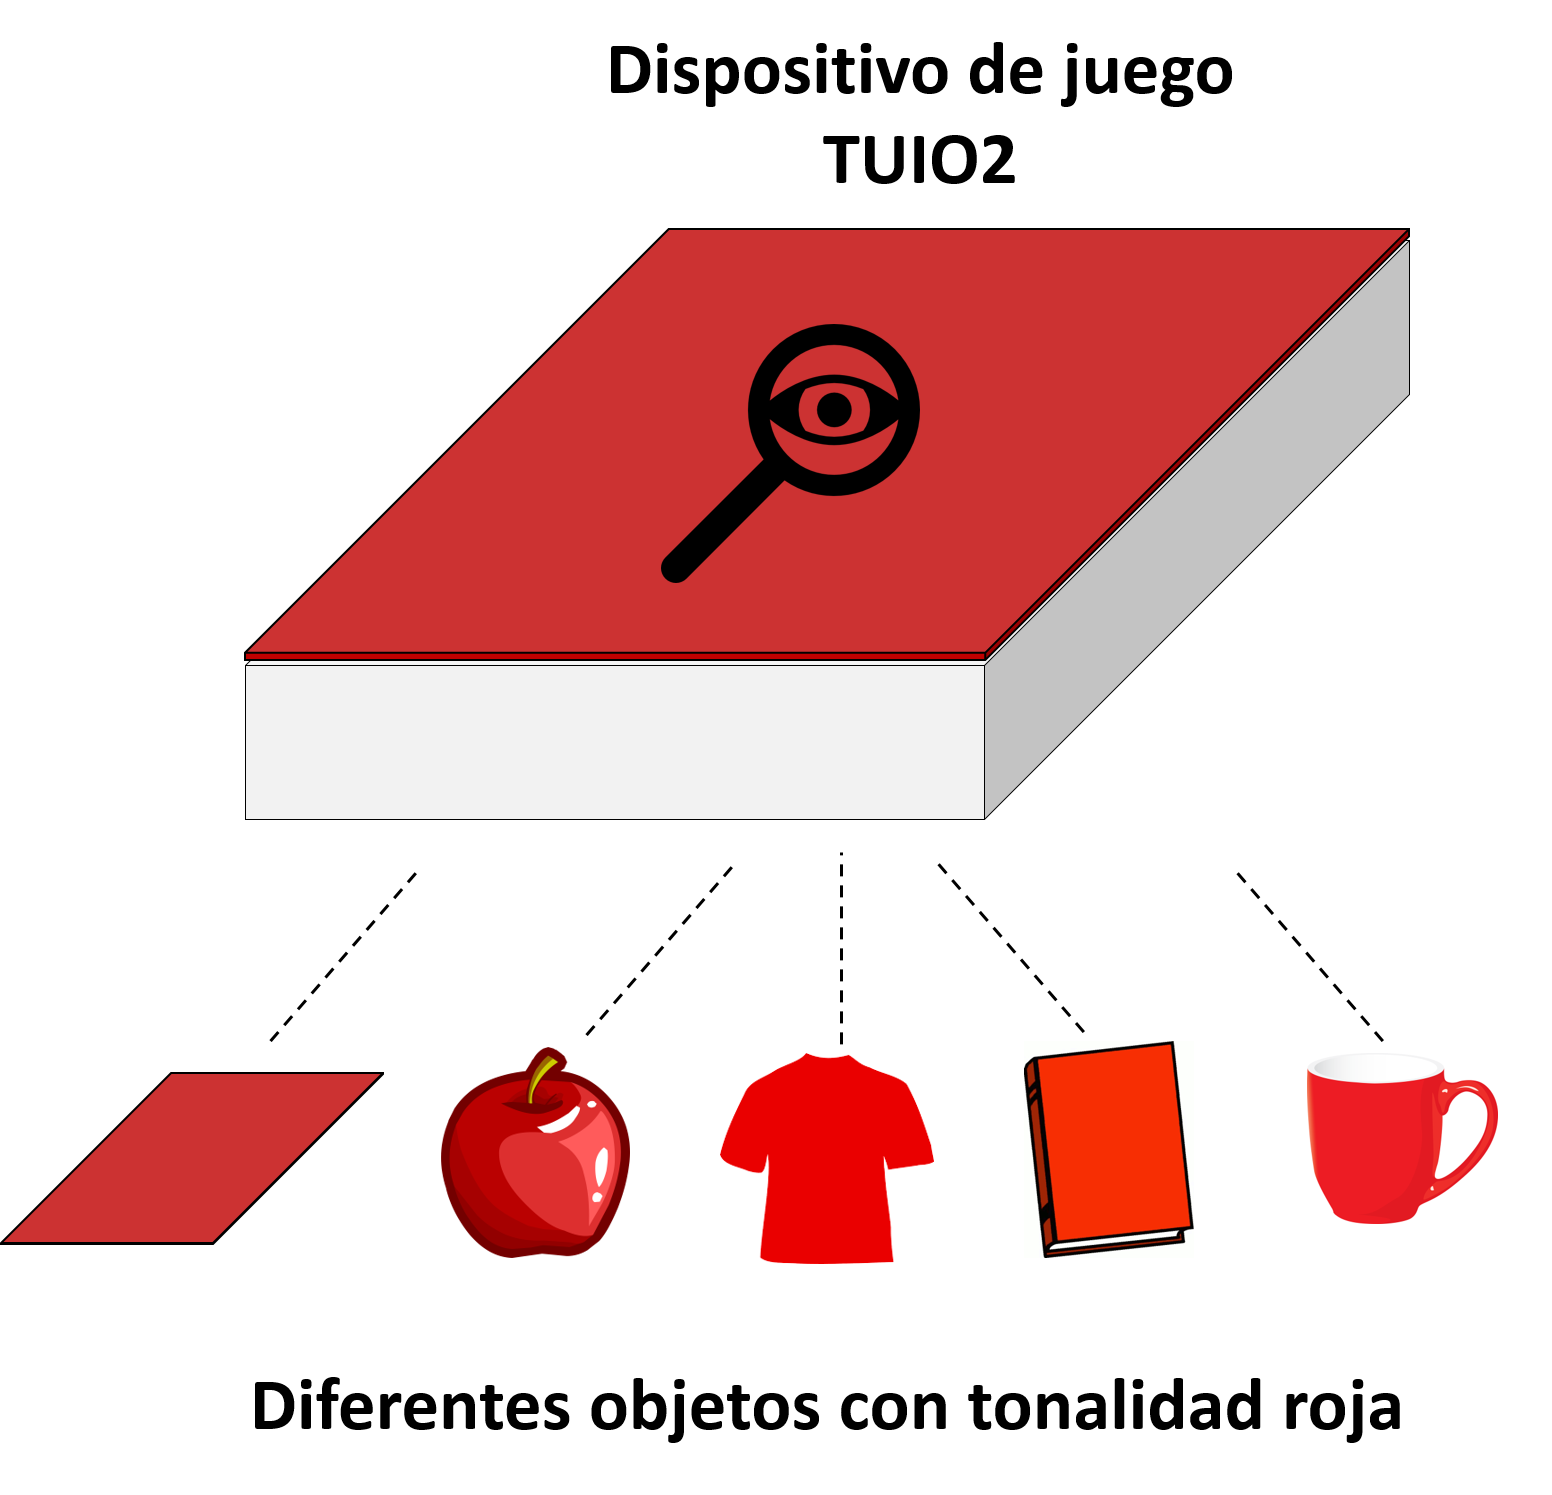
\includegraphics[width=0.7\textwidth]{TUIO_Color1.png}
\caption{Ejemplo de aplicación para detectar objetos color rojo mediante el sensor de color.}
\label{fig:TUIO_Color1}
\end{center}
\end{figure}



\textbf{Sistema operativo y lenguajes de programación. Herramientas software}
El sistema operativo utilizado en ambos dispositivos es \emph{Raspbian}.
\emph{Raspbian} es un sistema operativo basado en la distribución \emph{Debian}, recomendado para \emph{Raspberry Pi} por estar optimizado para su \emph{hardware}, siendo el más estable y con mayor rendimiento.
En esta distribución del sistema operativo, son instalados los paquetes necesarios para el intérprete \emph{Python} y \emph{Kivy}, que serán las herramientas utilizadas para realizar la programación de toda la plataforma de juego.

La documentación relacionada con la instalación de \emph{Raspbian}, se encuentra detallada en: \emph{Sección ~\ref{subs:raspbian} Sistema Operativo GNU/Linux. Raspbian.}


\subsubsection{Próximas historias de usuario.}
\begin{itemize}
\item Estructura de la aplicación.
\item Programa de pruebas comunicaciones entre dispositivos.
\end{itemize}


\subsection{Iteración 6: Estructura de la aplicación. Programa de pruebas comunicaciones entre dispositivos.}

\subsubsection{Organización y estructura de la aplicación.}

Antes de proceder a la programación de las aplicaciones, es necesario establecer una estructura para el proyecto, almacenando los archivos en distintos directorios, dependiendo de la función que realice cada uno de ellos (ver Figura ~\ref{fig:formato}).

El directorio principal de la aplicación es nombrado \texttt{itanium}. En este directorio se encuentra el archivo \texttt{Tuio1.py}, que es el módulo principal de la aplicación. Contiene el código en lenguaje \emph{Python}, donde se ejecutan los diferentes módulos, gestión de eventos, ejecución de la interfaz gráfica, etc. Dentro del directorio \texttt{itanium}, existen tres carpetas donde se organizan los diferentes archivos que dispone la aplicación:
\begin{itemize}
\item Carpeta \texttt{lib}, dedicada a las diferentes librerías creadas para el proyecto, como son las comunicaciones de servidor y sensores.
\item Carpeta \texttt{screens}. Incluye los archivos de extensión \emph{kv}. Estos archivos contienen el código (escritos en lenguaje \emph{Kivy}), de los distintos elementos y objetos que componen la interfaz gráfica de la aplicación (botones, figuras, fondos, etc..).
\item Carpeta \texttt{data}. En este directorio se encuentran las distintas imágenes utilizadas para la interfaz gráfica.
\end{itemize}

\begin{figure}[!h]
\begin{center}
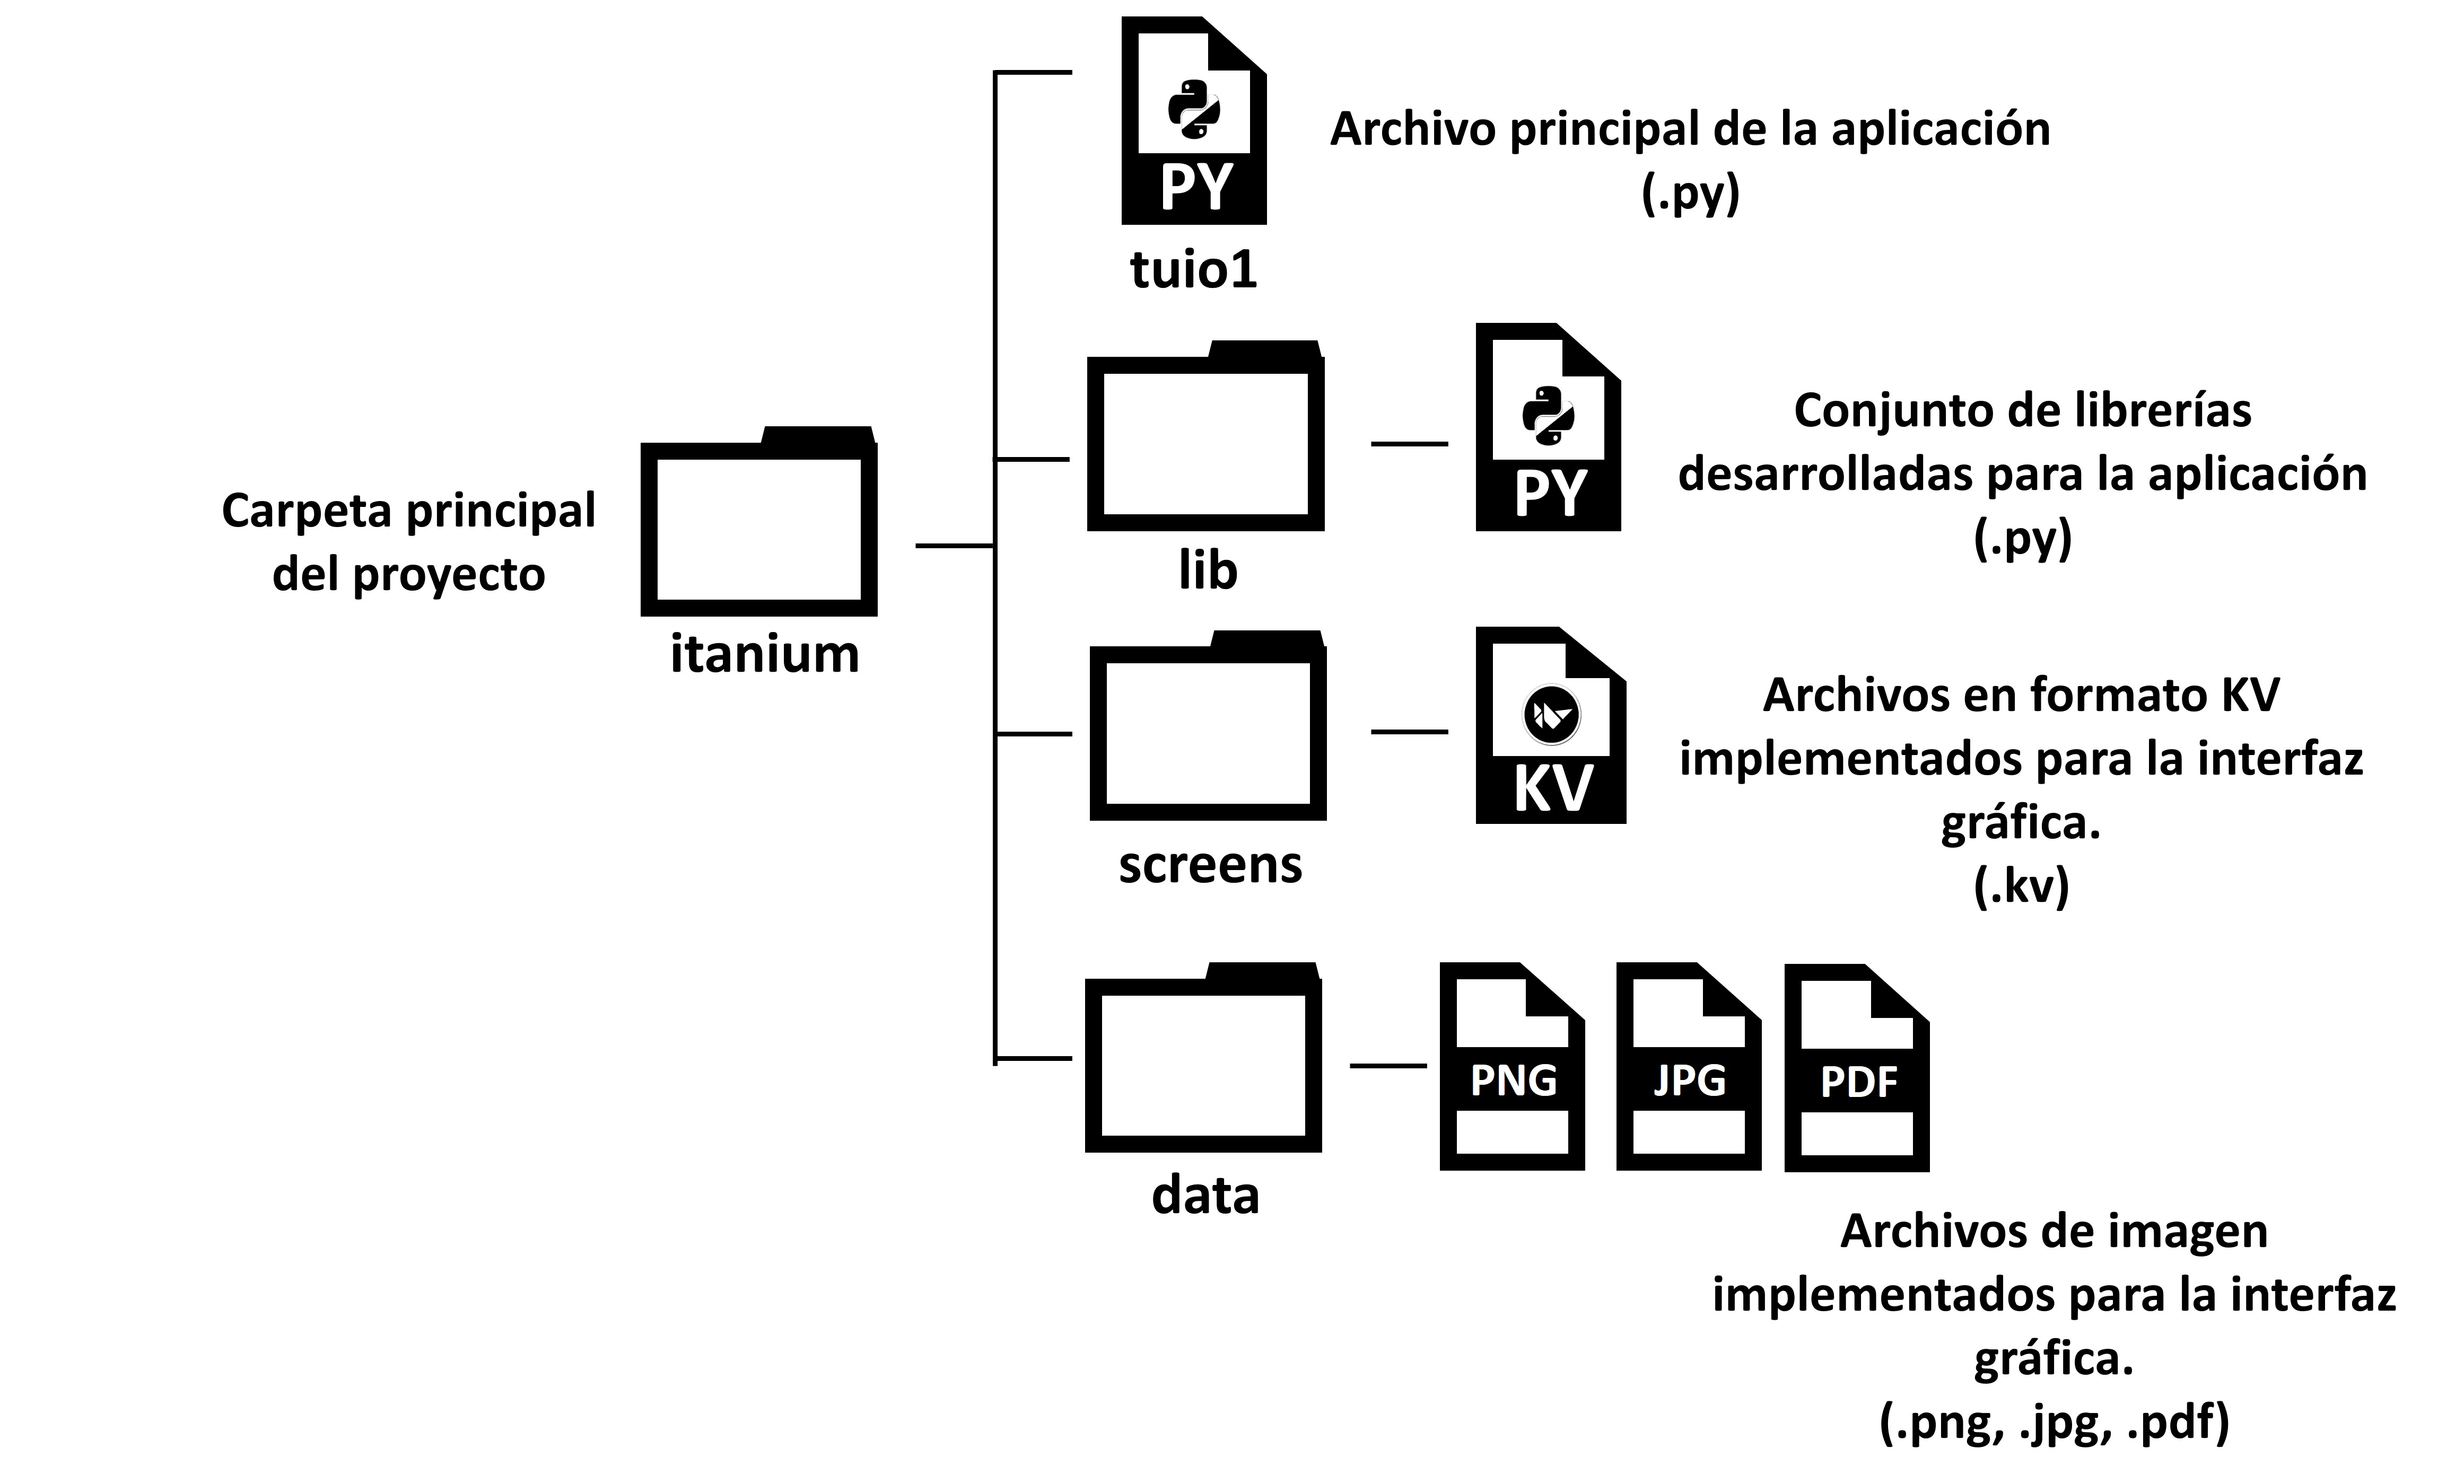
\includegraphics[width=0.7\textwidth]{formato.jpg}
\caption{Estructura de carpetas para la aplicación.}
\label{fig:formato}
\end{center}
\end{figure}


\subsubsection{Librerías para servidor y cliente.}
Las librerías utilizadas para crear las comunicaciones del lado servidor y cliente son:
\begin{itemize}
\item socket
\item Theread
\item struct
\item Queue
\end{itemize}

Las comunicaciones entre los dispositivos \emph{TUIO1} y \emph{TUIO2}, se realizan de manera inalámbrica (\emph{WiFi}), utilizando la librería \texttt{sockect}, con protocolo de comunicaciones \emph{TCP/IP}.
El dispositivo \emph{TUIO1} ejecuta el lado servidor, y \emph{TUIO2} el lado cliente.
Se establece la siguiente jerarquía: \textbf{el cliente solo enviará información a petición del servidor.}
Los mensajes de entrada/salida son almacenados en \emph{colas} (librería \texttt{Queue}), de una manera estructurada (librería \texttt{struct}, para generar eventos dentro del programa.
Tanto el cliente como el servidor administran los eventos mediante \emph{hilos} (librería \texttt{Thread}), que se ejecutan de forma paralela al resto del programa.


\subsubsection{Estructura básica servidor.}
La secuencia de operaciones básicas para el servidor son las siguientes:
\begin{itemize}
\item Crear un canal de comunicaciones. La llamada \emph{socket} asigna un descriptor de archivo a un canal de comunicación. Es necesario proporcionar datos sobre el dominio y tipo del conector. En este caso se emplea el protocolo \emph{IPv4} y un conector tipo \emph{STREAM}, que es el tipo de flujo que utiliza el protocolo \emph{TCP}, el cual asegura que los mensajes enviados al cliente llegan en el mismo orden en el cual fueron enviados.
\texttt{sock = socket(AF\_INET, SOCK\_STREAM)}
El objeto \texttt{sock} creado, implementa toda la \emph{API socket}.

\item Configurar direcciones origen/destino. El \emph{host} hace referencia a la dirección \emph{IP} del servidor, y \emph{port} al puerto de escucha para conexiones de entrada.
\texttt{sock.bind((host, port))}

\item Configurar el número de conexiones simultáneas, método \texttt{listen()}.
Solo es necesario una conexión simultánea.
\texttt{sock.listen(1)}

\item Crear un \emph{socket} esclavo para atender la conexión.
\texttt{client\_connection, client\_address = sock.accept()}
Se instancia el objeto \texttt{cliente\_connection}.

\item Recibir datos del cliente.
\texttt{client\_connection.recv(1024)}

\item Enviar datos al cliente.
(En este ejemplo es necesario introducir un mensaje por medio del teclado)
\texttt{client\_connection.send(input().encode('utf-8'))}

\item Cerrar el canal de comunicación.
\texttt{client\_connection.close()}
\end{itemize}


\subsubsection{Estructura básica cliente.}
La secuencia de operaciones básicas para el cliente son las siguientes:
\begin{itemize}
\item Crear un canal de comunicaciones. Al igual que el lado servidor, la llamada \emph{socket} asigna un descriptor de archivo a un canal de comunicación.
\texttt{sock = socket(AF\_INET, SOCK\_STREAM)}

\item Establecer dirección de destino con el método \texttt{conect()}, indicando los parámetros de dirección IP del servidor (\texttt{host}), y puerto de escucha (\texttt{port}.
\texttt{sock.conect(host,port)}

\item Recibir datos del servidor.
\texttt{client\_connection.recv(1024)}

\item Enviar datos al servidor.
(En este ejemplo es necesario introducir un mensaje por medio del teclado)
\texttt{client\_connection.send(input().encode('utf-8'))}\\

\item Cerrar el canal de comunicación.
\texttt{client\_connection.close()}
\end{itemize}

\subsubsection{Resultados programa de pruebas comunicaciones.}
Los resultados obtenidos referentes a las comunicaciones del lado cliente y servidor, al igual que el manejo de eventos en ambos dispositivos, son reflejados en: \emph{Capítulo \ref{chap:resultados} Resultados, en el apartado \ref{chap:comunicaciones} Comunicaciones cliente-servidor}.


\subsubsection{Próximas historias de usuario.}
\begin{itemize}
\item Inicio del sistema de localización entre dispositivos.
\end{itemize}



\subsection{Iteración 7: Inicio del sistema de localización entre dispositivos.}

\subsection{Iteración 8: Lectura de datos y diseño de máquina de estados de la unidad de medición inercial \emph{MPU9250}.}

\subsection{Iteración 9: Diseño software de las interfaces gráficas de usuario}

\subsection{Iteración 10: Diseño software de juego en la plataforma.}


\subsection{Iteración 11 Sistema de actualización software.}
